\documentclass[a4paperm]{article}
%\documentclass[12pt,twocolumn]{article}

\usepackage[T2A]{fontenc}
\usepackage[utf8]{inputenc}
\usepackage[russian,english]{babel}
\usepackage{amsmath,amsthm,amssymb,stackrel}
\usepackage[affil-it]{authblk}
\usepackage{cite}
\usepackage{scrextend}
\usepackage{verbatim}
\usepackage{paralist}
\usepackage[mediumspace,mediumqspace,Grey,squaren]{SIunits}
\addtokomafont{labelinglabel}{\sffamily}
\usepackage{amsmath}
\usepackage{graphicx}
 \usepackage[usenames, dvipsnames]{color}
 \usepackage{multirow}
 \usepackage{longtable}
 \usepackage{lineno}
 \usepackage{textcomp}
 
 \usepackage{xr}
 
 
%\usepackage[none]{hyphenat} %no nyphenation

\usepackage{SIunits}
\usepackage{miller}
\usepackage[version=3]{mhchem}

\usepackage{float} %H with figures

\setlength{\parindent}{5ex}

 \usepackage{newfloat} %For numbering of supplemmentary figures
 \DeclareFloatingEnvironment[name={Supplementary Figure}]{suppfigure}

\graphicspath{{figures/}}
\externaldocument{supplementary/smose_supp}

\usepackage[outdir=./]{epstopdf}

\begin{document}

%\linenumbers

\title{The Janus-structures of transition metal dichalcogenides with low enthalpy and new crystallchemistry}


\author[1,2,3]{Pavel N. Gavryushkin
   \thanks{Electronic address: \texttt{gavryushkin@igm.nsc.ru, p.gavryushkin@g.nsu.ru}; Corresponding author}}     
\author[2]{Nursultan Sagatov}
\author[1]{Ekaterina V. Sukhanova}
\author[1]{Zakhar I. Popov}
\author[4]{Inna Medrish}

\affil[1]{Emanuel Institute of Biochemical Physics of Russian Academy of Sciences, 4 Kosygin Street, Moscow, 119334, Russian Federation}
\affil[2]{Sobolev Institute of Geology and Mineralogy, Siberian Branch of Russian Academy of Sciences, prosp. acad. Koptyuga 3, 630090 Novosibirsk, Russian Federation}
\affil[3]{Novosibirsk State University, Pirogova 2, Novosibirsk 630090, Russian Federation}
\affil[4]{Samara Center for Theoretical Material Science (SCTMS), Samara State Technical University, Molodogvardeyskaya St. 244, Samara, Russia 443100}


\date{}
\maketitle

%\linenumbers

\begin{abstract}
Transition metal dichalcogenides (TMDs) like MoS2 or WS2 together with graphene and \textcolor{red}{its derivatives are most perspective and widely investigated 2D structures Захар замени это более подходящей фразой}.
TMDs with upper and lower layers of different chalcogen atoms were produced experimentally and was called Janus structures.
In the present work, we perform the theoretical search of the new Janus structures on the  wide range of TMDCs compounds and reveal new perspective structures.
Yanus structures of XTMY compositions, where X and Y are S, Se, Te, or O and TM is Mo, V, or W were considered.
Two of the found structures, called T-hor and airss-1 of SMoSe and SVSe compositions, are especially perspective for experimental synthesis and practical application.
These structures show dynamic stability and have enthalpies lower than enthalpy of experimentally synthesised although metastable 1T structure.
For  SVSe composition, enthalpy of airss-1 structure is 0.22 ev/f.u lower than that of 1T structure and 0.08  ev/f.u higher than that of  1H structure.
Presence of the vanadium atoms having magnetic moment in the crystal structure implies the possible practical application as \textcolor{red}{magnetic materials (?)}.
Also we revel several dynamically stable crystal structures with unique crystal chemistry which are important for the further crystallchemical design of the new TMDs structures, among them test-3 and airss-3 crystall structure.
Test-3 is characterised by the Mo dimers with Mo--Mo distance sufficiently lower than in any other structure of TMDs, just 2.2.\AA.
I the structure of airss-3, TM atoms are in the plane of chalcogen atoms and thus 3-layered sandwhich chalcogen--TM--chalcogen is transformed into two layered (chlcogen,TM)--(chalcogen,TM).


\end{abstract}

%%%%%%%%%%%%%%%%%%%%%%%%%%%%%%%%%%%%%
\section{Introduction}
%%%%%%%%%%%%%%%%%%%%%%%%%%%%%%%%%%%%%

Transition metal dichalcogenides (TMDs) represent a wide family of materials consisting of transition metal (TM: group IV, V or VI) surrounded by chalcogen atoms (Ch: S, Se or Te). 
TMDs crystallize in four main structural types including CdI2, MoS2 and FeS2 in pyrite-type and less frequently in marcasite-type structural types \cite{wells1986_book} [A.F. Wells. Structural Inorganic Chemistry, 1986]

The first two structural types are characterized by the layered structures with Ch-TM-Ch sandwiches bonded with each other by the weak Van-der-Waals bonds and, therefore, the crystals can be exfoliated into individual stable layers \cite{zhang2020intercalation}. These quasi-2D sandwiches attract considerable attention due to their wide range of properties \cite{li2017graphene, SHI20181, xi2016ising, hu2019recent, pi2019recent}. 
Particularly the TMDCs with TMCh2 stoichiometry can act as semiconductors \cite{nayeri2018transport}, metals \cite{zhao20212d}, semimetals \cite{xu2020high, zhao2020observation} or superconductors \cite{wang2020nodeless,hsu2017topological} which make family of TMDs suitable for a lot of applications. 

At ambient conditions MX2 (M=Mo,W, X=S,Se) structures crystallize in the archetype of molybdenite structure (MoS2) which consists of close-packed layers of chalcogen atoms placed exactly one under another along c-axis and TM atoms occupied the centers of half trigonal prismatic cavities located between the layers of chalcogen atoms. 
In the most stable polytype of molybdenite structure M--X--M multiplet layers similarly to {\it hcp} structure, which is close-packed structure with periodicity of stacking through each two layers, the structure has hexagonal symmetry and according to Ramsdell notation is denoted as 2H.
In the present work we consider isolated multiplet M--X--M layers, which are usually denoted as 1H.
Such a sandiwich, which in crystllchemical community usually termed as multiplet layer, we will call {\it monolayer}.
The last term is more accepted one in the field of 2D materials. 

If one layer of chalcogen atoms in M--X--M monolayer  layer is shifted, the coordination polyhedron of metal atoms changes from trigonal prism to the octahedron and the structure of CdI2 structural type is formed. 
The monolayer of such a structure has trigonal symmetry and will be designated as 1T \cite{huang2020recent}. 
The deformed 1T structure denoted as 1T' \cite{huang2020recent} will be also considered in the manuscript.
Depending on the exact chemical composition of the TMD monolayer, 1H or 1T phase is thermodynamically stable \cite{ataca2012stable}. 
For the disulphides (as well as diselenides and ditellurides) of Mo or W, the  1T-phase is less energetically favorable than 1H-phase with the same chemical composition. 
However 1T structure can be obtained metastably by means of intercalation \cite{kan2014structures, wang2014atomic}, deformation \cite{duerloo2014structural} or surface functionalization \cite{tang2015stabilization, voiry2015covalent}. 
In contrast to Mo, W and most of the other TMs, dichalcogenides of vanadium are not known \cite{murphy1977preparation, le1979elaboration}. 
However, VSe2 structure is known in the form of 2H structure with additional V atoms located in the centers of empty trigonal prisms between the sandwiches and have the composition of Se2V1.005 \cite{rigoult1982}.

Recently a new subclass of TMDs, the so-called Janus structures, where top and bottom layers are formed by different chalcogen atoms, were produced and attracts significant interest \cite{lu2017, zhang2017janus}. 
The opportunity to change the top layer of atoms opens an additional degree of freedom to manipulate the properties of TMDs. 
Janus TMDs have structural symmetry breaking \cite{li2017electronic, van2020first} resulting in Rashba spin splitting \cite{hu2018intrinsic} and transverse dipole moment leading to large piezoelectricity \cite{dong2017large, li2018recent}. 
The Janus structures of TMDs have a lot of potential applications, among which water-splitting \cite{xia2018universality, ma2018janus} or hydrogen evolution reaction \cite{er2018prediction, zhou2019janus}. 
Theoretical investigations show that, as in the case of pristine monolayers, Janus TMDs with different chemical compositions can be thermodynamically stable in the 1H and 1T structures desrcibed above
Meanwhile, the different composition of the upper and bottom layers assume the possibility for the stabilization of the new structures, substantially different from 1H or 1T.
This assumption was the motivation for us to perform the search for the new Janus TMDs structure with unbiased methods of crystal structure prediction, which have not been performed jet.




\begin{figure}[H]
        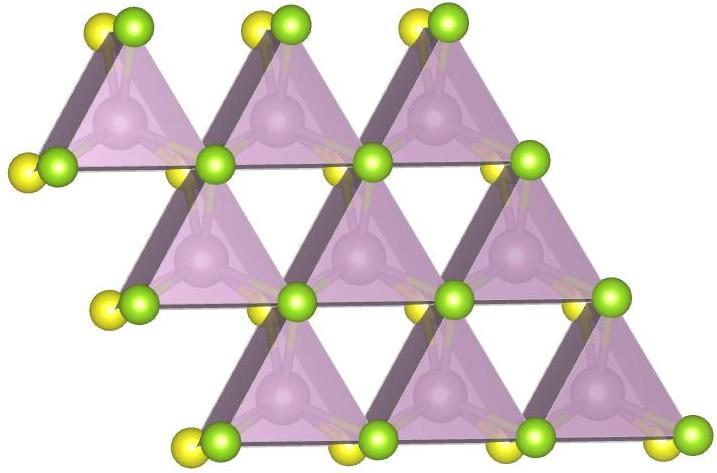
\includegraphics[width=0.4\textwidth]{1H.jpg}
        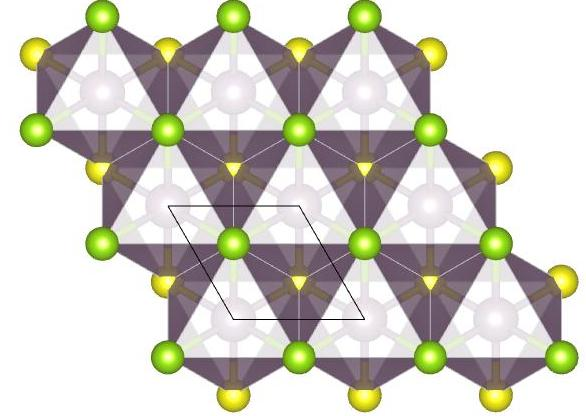
\includegraphics[width=0.4\textwidth]{1T.jpg}
        \caption{Packing of trigonal prisms and octahedra in H and T structures}
\label{1H1T}
\label{fes_fxt}
\end{figure}

\begin{figure}[H] \centering
	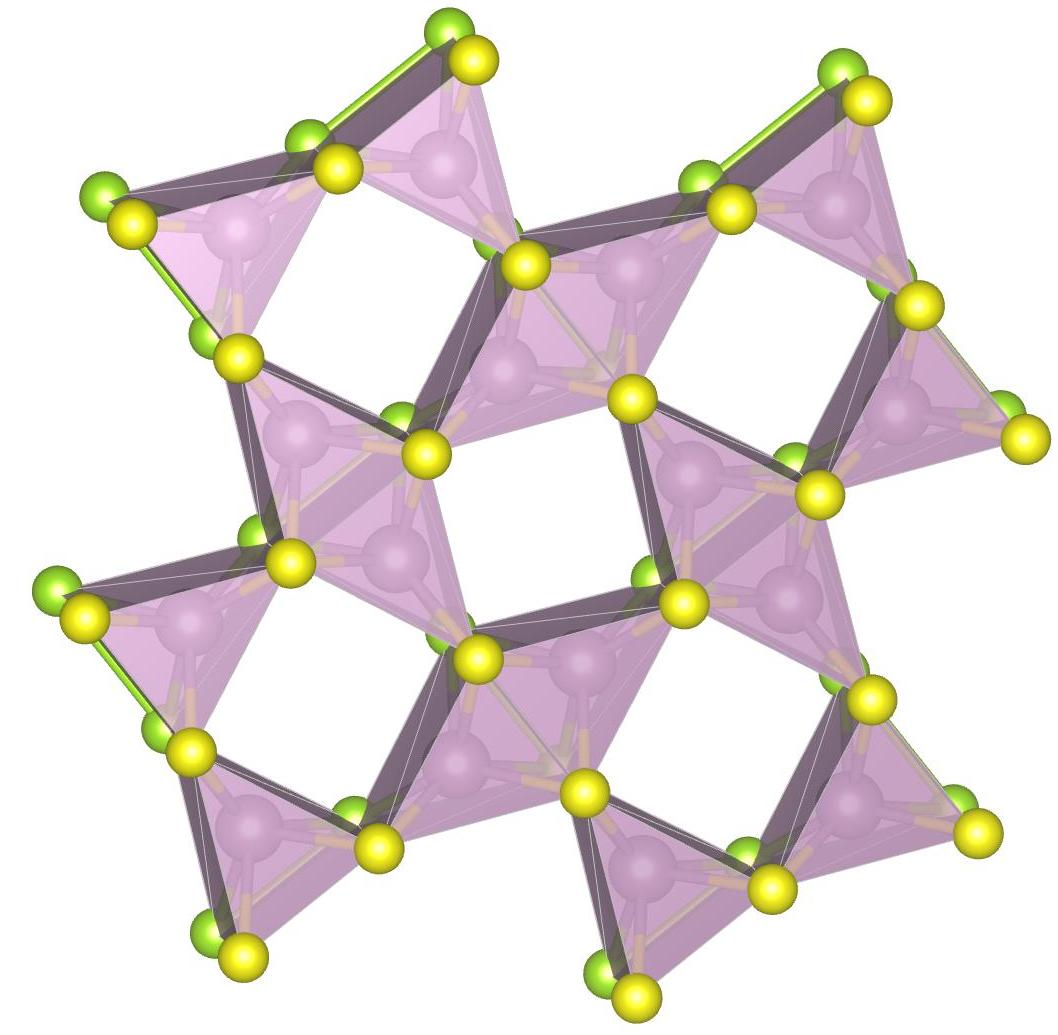
\includegraphics[width=0.4\textwidth]{fes_SMoSe.jpg}
        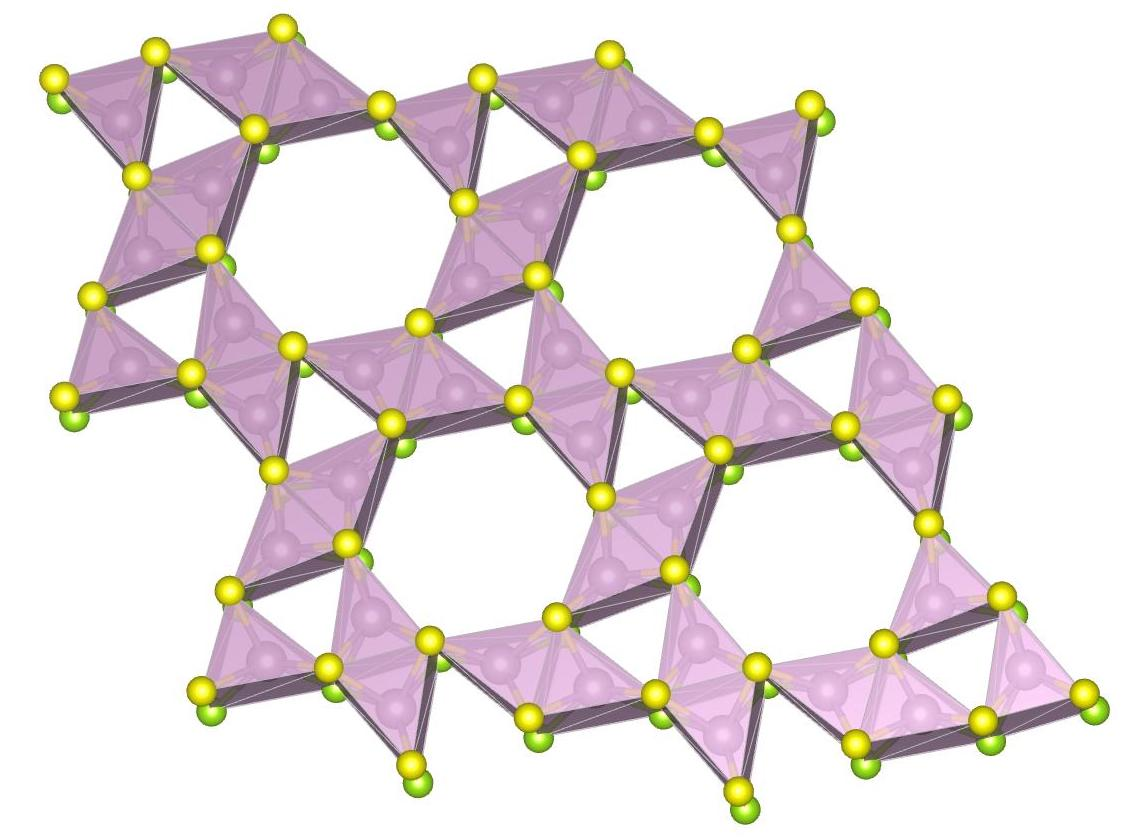
\includegraphics[width=0.5\textwidth]{fxt_SMoSe.jpg}
	\caption{Packing of trigonal prisms in fes and fxt structures.}
\label{fes_fxt}
\end{figure}

\begin{figure}[H] \centering
	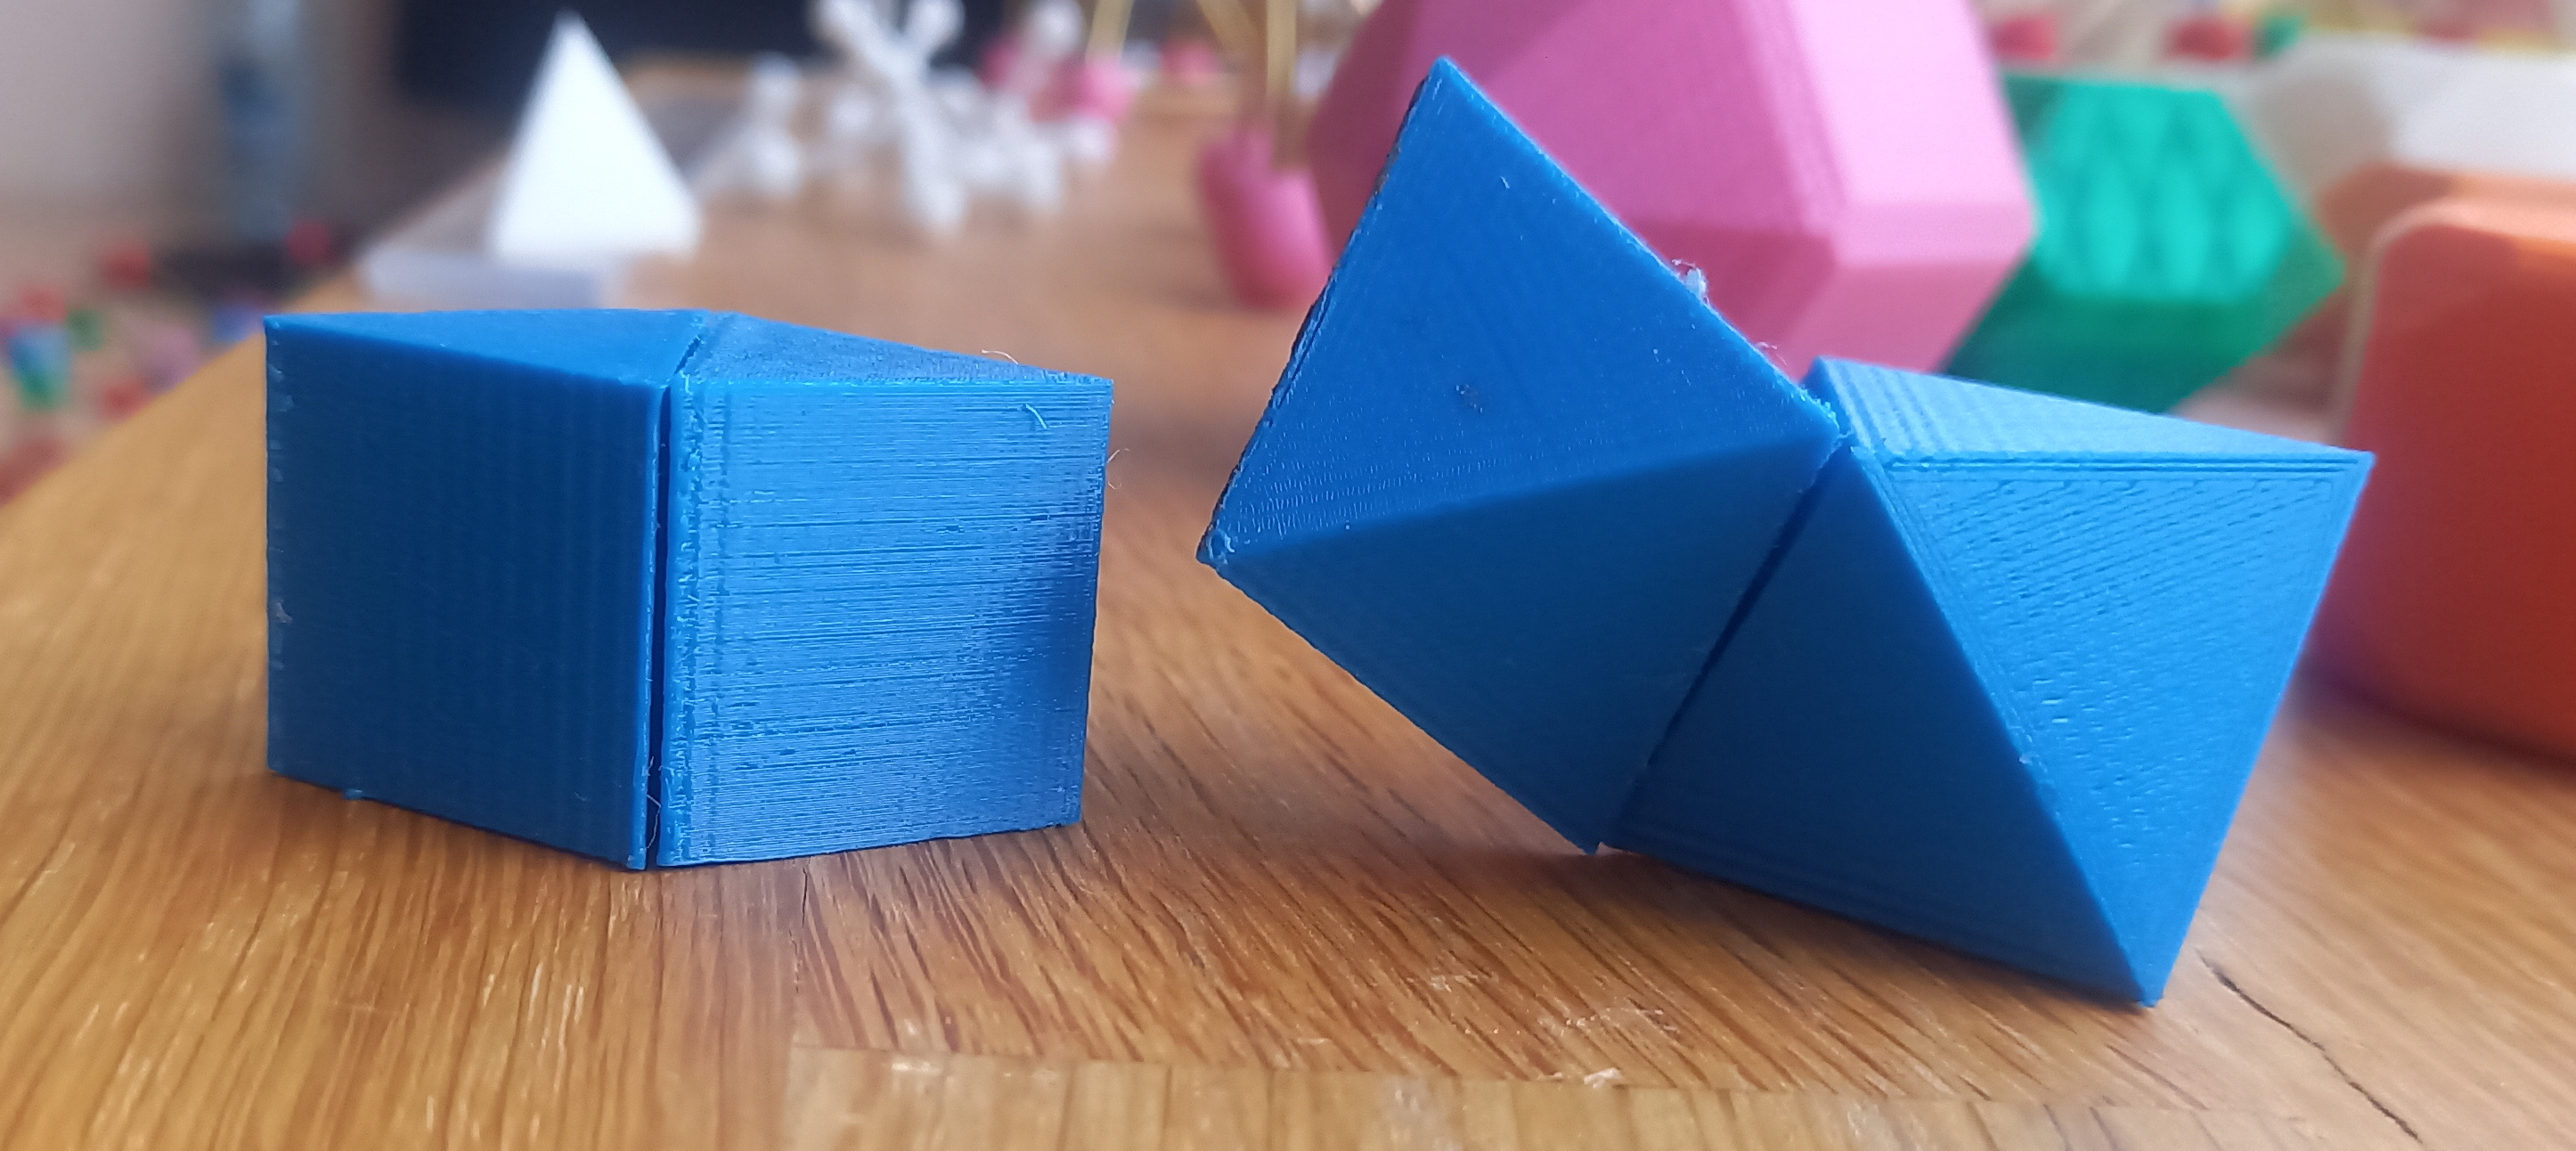
\includegraphics[width=0.5\textwidth]{2prism_oct.jpg}
	\caption{Two face-shared trigonal prisms and octahedra, the diviation from the horisontal plane in the last case is clearly visible}
\label{2prism_oct.jpg}
\end{figure}



%%%%%%%%%%%%%%%%%%%%%%%%%%%%%%%%%%%%%
		\section{Methods}
%%%%%%%%%%%%%%%%%%%%%%%%%%%%%%%%%%%%%

%%%%%%%%%
\subsection*{Crystal structure prediction}
%%%%%%%%%


The search for the lowest-enthalpy monolayer structures of SMSe (M = Mo, V) composition was performed using evolutionary algorithms implemented in the USPEX program package \cite{uspex1,uspex2,uspex3} and the random sampling method implemented in the AIRSS software \cite{airss1,airss2}.

The crystal structure search within USPEX was performed in fixed composition mode with 2--6 formula units per unit cell.
The number of structures in the first generation of the calculations was equal to 180.
50\% of the structures with the lowest enthalpy were selected after the optimization and then used to produce the next generation.
A new generation was produced as follow: 50\% of all structures were generated by heredity, 10\% -- by atomic mutation, 10\% –- by lattice mutation, and 30\% –- randomly.
In average, 40--47 generations were produced and relaxed.
Using AIRSS program about 5000--6000 structures were randomly generated and optimized for compounds with 4 and 6 formula units per unit cell and structures with the lowest enthalpy were selected.

The total energies and forces were calculated by solving the Schr\"{o}dinger equation based on projector augmented plane-wave implementation \cite{blochl1994projector} of density functional theory (DFT) using the VASP program package \cite{vasp1,vasp2}.
Exchange correlation effects were treated in the generalized gradient approximation (GGA) with Perdew-B\"{u}rke-Ernzerhof scheme \cite{pbe}.

In all crystal structure prediction calculations medium-quality optimization was performed using the conjugate gradient method \cite{conjugate_gradient}. 
The energy cutoff of plane waves was set to 420 eV and 700 eV for the intermediate structures and then for the most promising of them. 
The first Brillouin zone was sampled according to Monkhorst-Pack scheme \cite{monkhorst1976special} with the density of k-point being equal to 0.5 \AA$^{-1}$ and 0.2 \AA$^{-1}$, respectively. 
% проверить 2pi

To study a dynamic stability of predicted structures phonon dispersion spectra were calculated within the PHONOPY code \cite{phonopy}. 
We used VESTA program for crystal structures visualization and figures preparation \cite{momma2011vesta}.
\textcolor{red}{Instruments of Bilbao Crystallographic server have been used for the structures symmetrisation \cite{}}


%%%%%%%%
\subsection*{Topological search}
%%%%%%%%

Original crystal-structural information was selected from the Inorganic Crystal Structure Database (ICSD, release 2020/2) \cite{icsd_1} and Cambridge Structural Database (CSD, release 2021) \cite{icsd_2}.

The procedures of screening of structural-graphic data bases of compounds by the methods of the combined geometric-topological analysis with ToposPro (http://topospro.com) package have been used \cite{topos_1}. 
We use bold three-letter symbols of the Reticular Chemistry Structure Resource nomenclature (for the three-letter nomenclature of polyhedral and nets see Reticular Chemistry Structure Resource, http://rcsr.anu.edu.au/, and \cite{rcsr} or ToposPro NDk-n symbols \cite{rcsr_2}) to designate the topological types of the underlying nets. 
The topology of an underlying net is determined in an automated mode by comparison of a set of topological indices of the net with those for the reference nets from the ToposPro TTD collection \cite{TTD}.

For the topological analysis we have used only fully solved crystal structures , without errors in the determination of interatomic bonds or chemical composition,
The nets of interatomic bonds were determined by the Domains methods with the program AutoCN \cite{blatov2016_rods}. 
Only strong interatomic bonds  with solid angles of the faces of Voronoi-Dirihle polyhedron $\Omega \geq 5 $ of the whole 4$\pi$ solid angle were considered.
Structures with the great values of unit cell parameters were excluded from the consideration.
For instance, we did not consider polytypes of ZnS with cell parameters more than 50 \AA.

Earlier the numerous structural relations between unhydrous simple salts and even more simple binary inorganic compounds have been shown \cite{blatov2011_salts, medrish2020_zintl}. 
Due to this well-known structural phenomena, we analyse topology not only for the complete  representation, but all so the topology of the underlying net.
In the complete representation, the net corresponds to the interatomic bonds of all strong bonds, while the underlying net is determined between metalls and centers of ligands.

Due to the short interatomic bonds, the topologies were not determined for the crystal structures airss1, fxt, and  test3.


%%%%%%%%%%%%%%%%%%%%%%%%%%%%%%%%%%%%%
			\section{Results}
%%%%%%%%%%%%%%%%%%%%%%%%%%%%%%%%%%%%%

\subsection*{Earlier known MX$_2$ structures and their enthalpies}

Although H and T structures are characterized by the different coordination polyhedra, they are similar in the manner of their interconnection.
The H structure consists of trigonal prisms [MX$_6$] ([MX$_3$Y$_3$] for Janus structures), and T structure – of the [MX$_6$] octahedra (Figure\ref{1H1T}).
Each trigonal prism share all three vertical edges with the neighbouring prisms and does not share any faces.
As the result, each vertex and each vertical edge of the trigonal prism is common for three prisms (Figure \ref{1H1T}).
Similarly in T structure, each octahedron share all edges inclined to the plane of sulphur atoms with neighbouring octahedra, and each vertex is common for three octahedra (Figure \ref{1H1T}).
Bond valence of Mo--S bond is nearly equal to +4/6 and there are necessary three such a bonds to compensate negative charge of S$2{2-}$.
Interconnection through the faces gives shorter bonds high-charged M$^{4+}$ ions, increasing the energy of Couloumb interaction, and making the structure less favourable \cite{pauling1929}.
As we will shown below the interconnection through the faces is also realised for predicted structures, although in most of the found structures coordination polyhedra share only common edges.

According to the performed calculations, 1H structure is the most favourable for SMoSe composition, but it is less favourable than 1T and 1T for SVSe composition.
The difference of enthalpies $H(1H)-H(1T)$ is equal to -0.73 ev/f.u. for SMoSe and 0.09 for SVSe (Table \ref{t:enthalpy}).
For SVSe composition the most favourable phase is 1T', the deformed analogue of 1T, which enthalpy is 0.11 ev/f.u lower than the enthalpy of 1T Table \ref{t:enthalpy}. 

The recently found fes and fxt structures are also characterised by the trigonal prismatic coordination.
However, in these structure prisms are connected not only through edges but also through the faces.
The structure can be built by means of connecting through the vertices double (edge-connected) trigonal prisms (Figure \ref{2prism_oct}b).
In accordance with above consideration, the enthalpies of fxt and fes structures are higher than that of 1H structure, although lower than that of 1T structures.
As well as in 1H and 1T structures, in fxt and fes structures,  each chalcogen atoms is connected to three atoms of transition metal, providing the local charge balance (Figure \ref{2prism_oct}b).
As we will show below this is also not the obligatory requirement and some of the predicted structures are not charactersied by the local charge balance.
According to our calculations, fes and fxt structures are close in enthalpy values.
For both SMoSe and SVSe, fes is more energetically favourable than fxt, with enthalpies difference equal to 0.01 ev/f.u. for SMoSe and 0.06 ev/f.u. for SVSe.
In turn, enthalpy of SMoSe-fes structure is 0.79 eV/f.u. higher than enthalpy of the 1H structure.
Enthalpy of SVSe-fex is 0.64 higher than enthaly of 1T'.
According to our calculations, the fxt and fes structures are less favourable than 1T structure, which was obtained experimentally, despite its metastability.
\textcolor{red}{The last fact contradicts to the earlier results according to which the fxt (fes?) structure if more favourable than 1T \cite{}. Поправьте меня если я не прав, Я точно помню эту фразу в статье по fxt или fes, но не смог найти статью}

1H and 1T structures provide the most uniform distribution of the chalсogen and transition metall atoms. 
Both nets of transition metall atoms and chalcogen atoms consist of the geometrically equal triangular rings.
Edge-sharing interconnection of trigonal prisms realised in fxt and fes structures inevitably results in the appearance of the cavities bigger than that in 1H and 1T structures. 
In fes structure the cavities have the form of the slightly compressed cube (Figure \ref{fes_SMoSe}).
The volume of these cavities is almost two times larger than the volume of the cavities in 1H structure (38.8 against 17.7 \AA$^3$).
In case of fxt structure, the volume of hexagonal cavities (Figure \ref{fxt_SMoSe} is almost 8 times larger than that in 1H structure (137.8 against 17.7 \AA$^3$).
In contrast to trigonal prisms, the face-sharing of the right octahedra seems to be problematic for quasi 2D structure, as it is results in the deviation from the flat arrangement (Figure\ref{2prism_oct}b -- supplementary).
However, as it will be shown below, the dynamically stable quasi 2D structure structures with face sharing octahedra coordination polyhedrons can be also produced.



%%%%%%%%%%%%%%%%%%%%%%%%%%%%%%%%%%%%%
		\subsection{New TMD structures}
%%%%%%%%%%%%%%%%%%%%%%%%%%%%%%%%%%%%%

Table \ref{t:enthalpy} shows the values of enthalpies for the most energetically favorable structures among revealed with USPEX and AIRSS, and Figures \ref{phon_smose} and  \ref{phon_svse} their phonon spectra. 
Among the found structures, two structures, T-hor and airss-1, are most promising.
In addition to dynamic stability, the enthalpies of formation of these structures are lower experimentally synthesised 1T phase.
This assumes the possibility for their experimental synthesis with nearly the same probability.

Crystal structures test-1, test-3, H-hor and airss-3 are dynamically stable for some of the considered compositions (Figures \ref{phon_smose} and  \ref{phon_svse}) but they are characterized by the enthalpies lower than that of 1T structure (Table \ref{t:enthalpy}. 
Crystal structure test-2 dynamically unstable (Figures \ref{phon_smose} and \ref{phon_svse}) although it preserves the initial geometry and symmetry after optimization.
However, the enthalpy of the structure is lower than that of SMoSe-1T  (Table \ref{t:enthalpy}).

Two dynamically stable (Figures \ref{phon_smose} and  \ref{phon_svse}) but energetically unfavorable (Table \ref{t:enthalpy}) structures called test-1 and test-3 were revealed.

Below we first consider the most promising T-hor and airss-1 crystal structures and then all other crystal structures which are important for crystallchamical design of the other 2D TMD structures.



\begin{table}[H]
	\caption{Calculated enthalpies of SMoSe and SVSe structures.} \label{t:enthalpy} \vspace{2mm}
	\centering
	\begin{tabular}{l*{5}{l}}
		\hline \hline
		\multirow{2}*{Phase} & \multicolumn{2}{c}{Enthalpy (eV/f.u.)} & \multicolumn{2}{c}{Relative H (eV/f.u.)}	\\
		\cline{2-3} \cline{4-5}
		& SMoSe & SVSe & SMoSe & SVSe\\
		\hline    		
		1H	&	-20.8588	&	-15.7908	&	0.0000	&	0.2022	\\
		1T	&	-20.1229	&	-15.8817	&	0.7358	&	0.1113	\\
		1T'	&	-20.4272	&	-15.9930	&	0.4315	&	0.0000	\\
		fes	&	-20.0677	&	-15.3545	&	0.7910	&	0.6385	\\
		fxt	&	-20.0572	&	-15.2915	&	0.8016	&	0.7015	\\
		test-1	&	-19.7876	&	-15.2359	&	1.0711	&	0.7571	\\
		test-2	&	-20.2611	&	-15.4713	&	0.5977	&	0.5217	\\
		test-3	&	-19.9359	&	-15.5461	&	0.9229	&	0.4468	\\
		H-hor	&	-20.0648	&	-15.7256	&	0.7939	&	0.2674	\\
		T-hor	&	-20.3004	&	-15.9091	&	0.5584	&	0.0838	\\
		airss-1	&	-20.2308	&	-15.6641	&	0.6280	&	0.3289	\\
		airss-3	&	-19.6106    &	-15.6467	&	1.2481 	&	0.3463	\\
		
		\hline \hline
	\end{tabular}
\end{table}


\begin{figure}[H]
	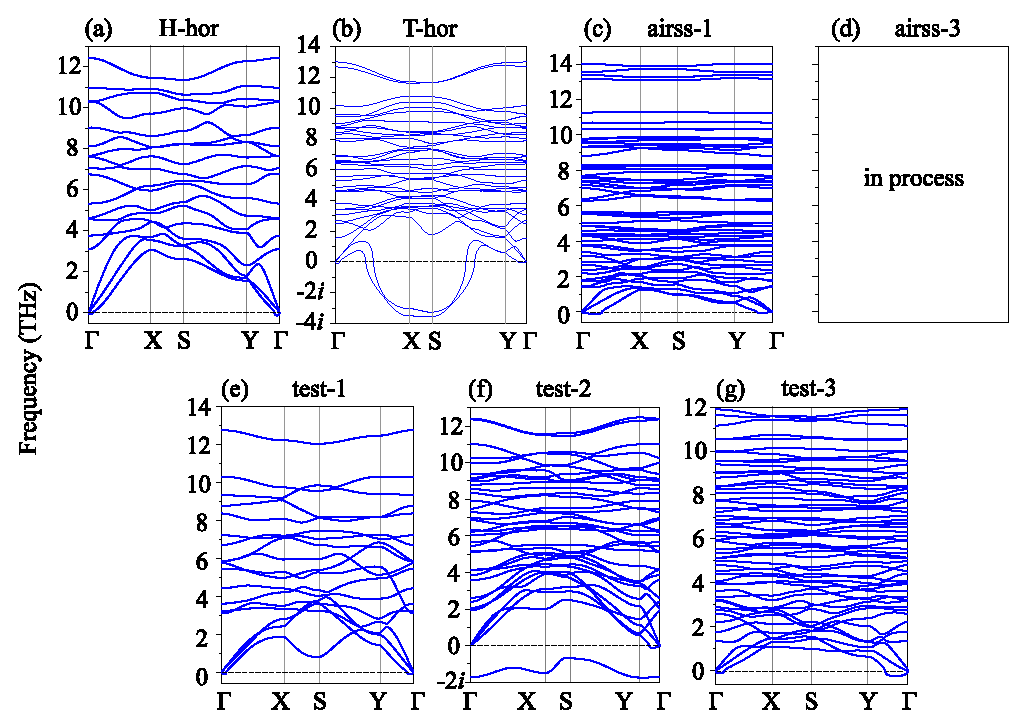
\includegraphics[width=\textwidth]{phon_smose.eps}
	\caption{Phonon dispersion curves of SMoSe structures. }
	\label{phon_smose}
\end{figure}

\begin{figure}[H]
	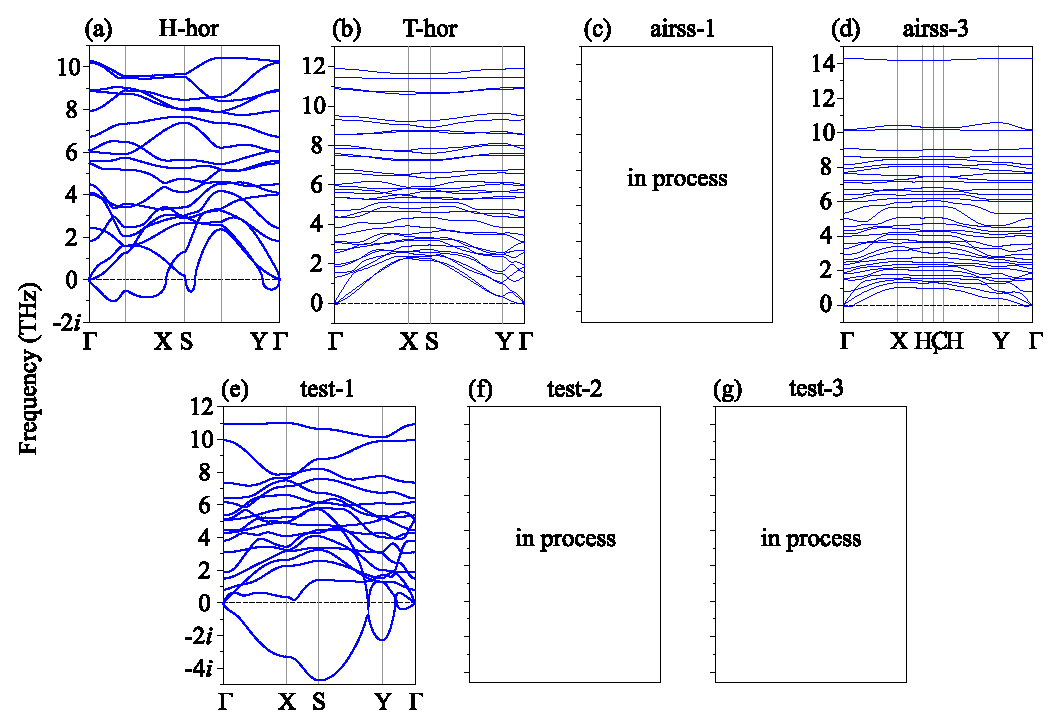
\includegraphics[width=\textwidth]{phon_svse.eps}
	\caption{Phonon dispersion curves of SVSe structures. }
	\label{phon_svse}
\end{figure}


\begin{table}[H]
    \small
	\caption{Predicted structures of SMoSe and SVSe} \label{t:str} \vspace{2mm}
	\centering
	\begin{tabular}{l*{9}{l}}
		\hline
		\multirow{2}*{Phase}	& 	\multirow{2}*{Space group}	& \multicolumn{3}{c}{\multirow{2}*{Lattice parameters (\AA, deg)}}	&	\multirow{2}*{Atom}	&	\multicolumn{3}{c}{Coordinates} \\ 
		\cline{7-9}
		&&&&&&  x	&	y	&	z \\ 
		\hline 
		SMoSe & $P1\ (\#1)$  &	$a=6.5969$ & $b=9.9921$ & $c=27.6937$  & Mo  &0.1478 &0.0694  &0.3275 \\
		airss-1&&$\alpha$ = 90.024& $\beta$=87.689& $\gamma$ = 89.999& Mo &0.641 &0.116 &0.165\\
		&&&&&	Mo	&	0.7221	&	0.0694	&	0.3275	\\
		&&&&&	Mo	&	0.6522	&	0.5690	&	0.3013	\\
		&&&&&	Mo	&	0.4381	&	0.8084	&	0.3090	\\
		&&&&&	Mo	&	0.9362	&	0.3069	&	0.3201	\\
		&&&&&	S	&	0.4283	&	0.6344	&	0.3668	\\
		&&&&&	S	&	0.6622	&	0.2613	&	0.3706	\\
		&&&&&	S	&	0.1931	&	0.2613	&	0.3706	\\
		&&&&&	S	&	0.9297	&	0.5373	&	0.3583	\\
		&&&&&	S	&	0.4270	&	0.9651	&	0.3745	\\
		&&&&&	S	&	0.9269	&	0.9415	&	0.3749	\\
		&&&&&	Se	&	0.9470	&	0.1309	&	0.2562	\\
		&&&&&	Se	&	0.7177	&	0.7655	&	0.2526	\\
		&&&&&	Se	&	0.1776	&	0.7655	&	0.2526	\\
		&&&&&	Se	&	0.4456	&	0.0464	&	0.2644	\\
		&&&&&	Se	&	0.9485	&	0.4613	&	0.2478	\\
		&&&&&	Se	&	0.4483	&	0.4348	&	0.2488	\\
		\hline 
		SMoSe & $Pm\ (\#6)$  &	$a=6.2189$ & $b=3.2228$ & $c=16.7225$  & Mo	&	0.5174	&	0	&	0.5164	\\
		H-hor&   &$\alpha$ = 90.000& $\beta$=98.670& $\gamma$ = 90.000& Mo	&	-0.0928	&	0.5	&	0.4739	\\
		&&&&& S	&	0.1525	&	0	&	0.4276	\\
		&&&&& S	&	0.6730	&	0	&	0.3962	\\
		&&&&& Se	&	0.7587	&	0.5	&	0.6054	\\
		&&&&& Se	&	0.2676	&	0.5	&	0.5806	\\
		\hline
		SVSe & $Pm\ (\#6)$  &	$a=3.6955$ & $b=12.0193$ & $c=17.1112$  & V	&	0.0921	&	0.3413	&	0.4568	\\
		T-hor&&$\alpha$ = 90.000& $\beta$=90.605& $\gamma$ = 90.000& V	&	0.5882	&	0.8456	&	0.5342	\\
		&&&&&	S	&	0.6057	&	0.7696	&	0.4077	\\
		&&&&&	S	&	0.0633	&	0		&	0.5125	\\
		&&&&&	S	&	0.3174	&	0.5		&	0.3765	\\
		&&&&&	Se	&	0.1058	&	0.2737	&	0.5943	\\
		&&&&&	Se	&	0.5950	&	0.5		&	0.4940	\\
		&&&&&	Se	&	0.8148	&	0		&	0.6313	\\
		\hline
		SVSe & $P1\ (\#1)$  &	$a=5.0351$ & $b=8.7721$ & $c=18.0178$  & V	&	0.2426	&	-0.0280	&	0.5623	\\
		airss-3&&$\alpha$ = 77.990& $\beta$=82.386& $\gamma$ = 78.789  & V	&	0.7676	&	0.0298	&	0.4302	\\		
		&&&&&	V	&	0.1205	&	0.3274	&	0.4532	\\
		&&&&&	V	&	0.8752	&	0.6755	&	0.5417	\\
		&&&&&	S	&	0.2587	&	0.0491	&	0.4287	\\
		&&&&&	S	&	0.7713	&	0.7610	&	0.4083	\\
		&&&&&	S	&	0.6782	&	0.3075	&	0.4066	\\
		&&&&&	S	&	0.1493	&	0.6174	&	0.4231	\\
		&&&&&	Se	&	0.7462	&	-0.0417	&	0.5734	\\
		&&&&&	Se	&	0.2518	&	0.2363	&	0.5951	\\
		&&&&&	Se	&	0.3271	&	0.6790	&	0.5997	\\
		&&&&&	Se	&	0.8115	&	0.3867	&	0.5779	\\
		\hline
	\end{tabular}
\end{table}


%%%%%%%%%%%%%%%%%%%%%%%%
\subsubsection{T-hor and airss-1 crystal structures}
%%%%%%%%%%%%%%%%%%%%%%%
T-hor structure was predicted using USPEX for VSSe, and for this composition it is more  enerheticaly favourable than bh 1H and 1T structure, although it is less favourable than 1T' (Figure \ref{t:enthalpy}).
Based on the VSSe-T-hor, the MoSSe-T-hor structure was constructed.
For MoSSe-T-hor is more favourable than 1T, although less favourable than 1H and 1T' (Figure \ref{t:enthalpy}).

Crystallchemically T-hor structure is similar to the 1T structure.
Both structures are characterised by octahedral coordination polyhedrons around TM atoms.
The difference is in the arrangement of this octahedra.
As it was mentioned, in 1T structure octahedra share only common edges, while in T-hor both edges and faces.
Both structures can be described within modular approach.
In this case, the module is the double row of octahedra connected through common edges.
This is, for instance, double cow consisting of the rows 2 and 3 on the Figure \ref{T_hor_T}.
The adjacent double layer (rows 4 and 5) are attached through the common faces  of the octahedra in T-hor structure (the face ABC on the Figure \ref{T_hor_T}) and though the common edge B'C' in 1T structure (the edge B'C' Figure \ref{T_hor_T}) as it is illustrated on Figure \ref{T_hor_slabs}.
The joining of the double layers through the common face is identical to the mirror reflection of the initial double layer in the plane going through this face.
This let to consider T-hor structure as the ordered polysyntheitic twin of 1T structure.

The described rearrangement of coordination octahedra results in the sufficient rearrangement of V atoms, with the appaearance of the zig-zag chain of V atoms connected by the shorter bonds (Figure \ref{T_hor_V}).
The nets of chalcogen atoms are not affected to much and in T-hor structure it is topologically the same as that in 1T structure, although the difference of geometrical parameters is sufficient (Figure \ref{T_hor_hcb}).
The angles between S--S bonds in VSSe-T-hor structure vary in the range 91.38-139.8\textdegree, while in VS2-1T structure all the angles are equal to 120\textdegree.
The S--S bond lengths in T-hor are in the range 3.45--3.87\AA, while in 1T all they are equal to 3.41 \AA.

T-hor structure is characterised by the uniqe topology– 3,3,5,8-coordinated net if short V--V bonds are considered and 3,3,5,6-coordinated net if V--V bonds are not considered.

The fact that H(1T)<H(T-hor)<H(1T') suggest the possibility for the formation

\begin{figure}[H]
        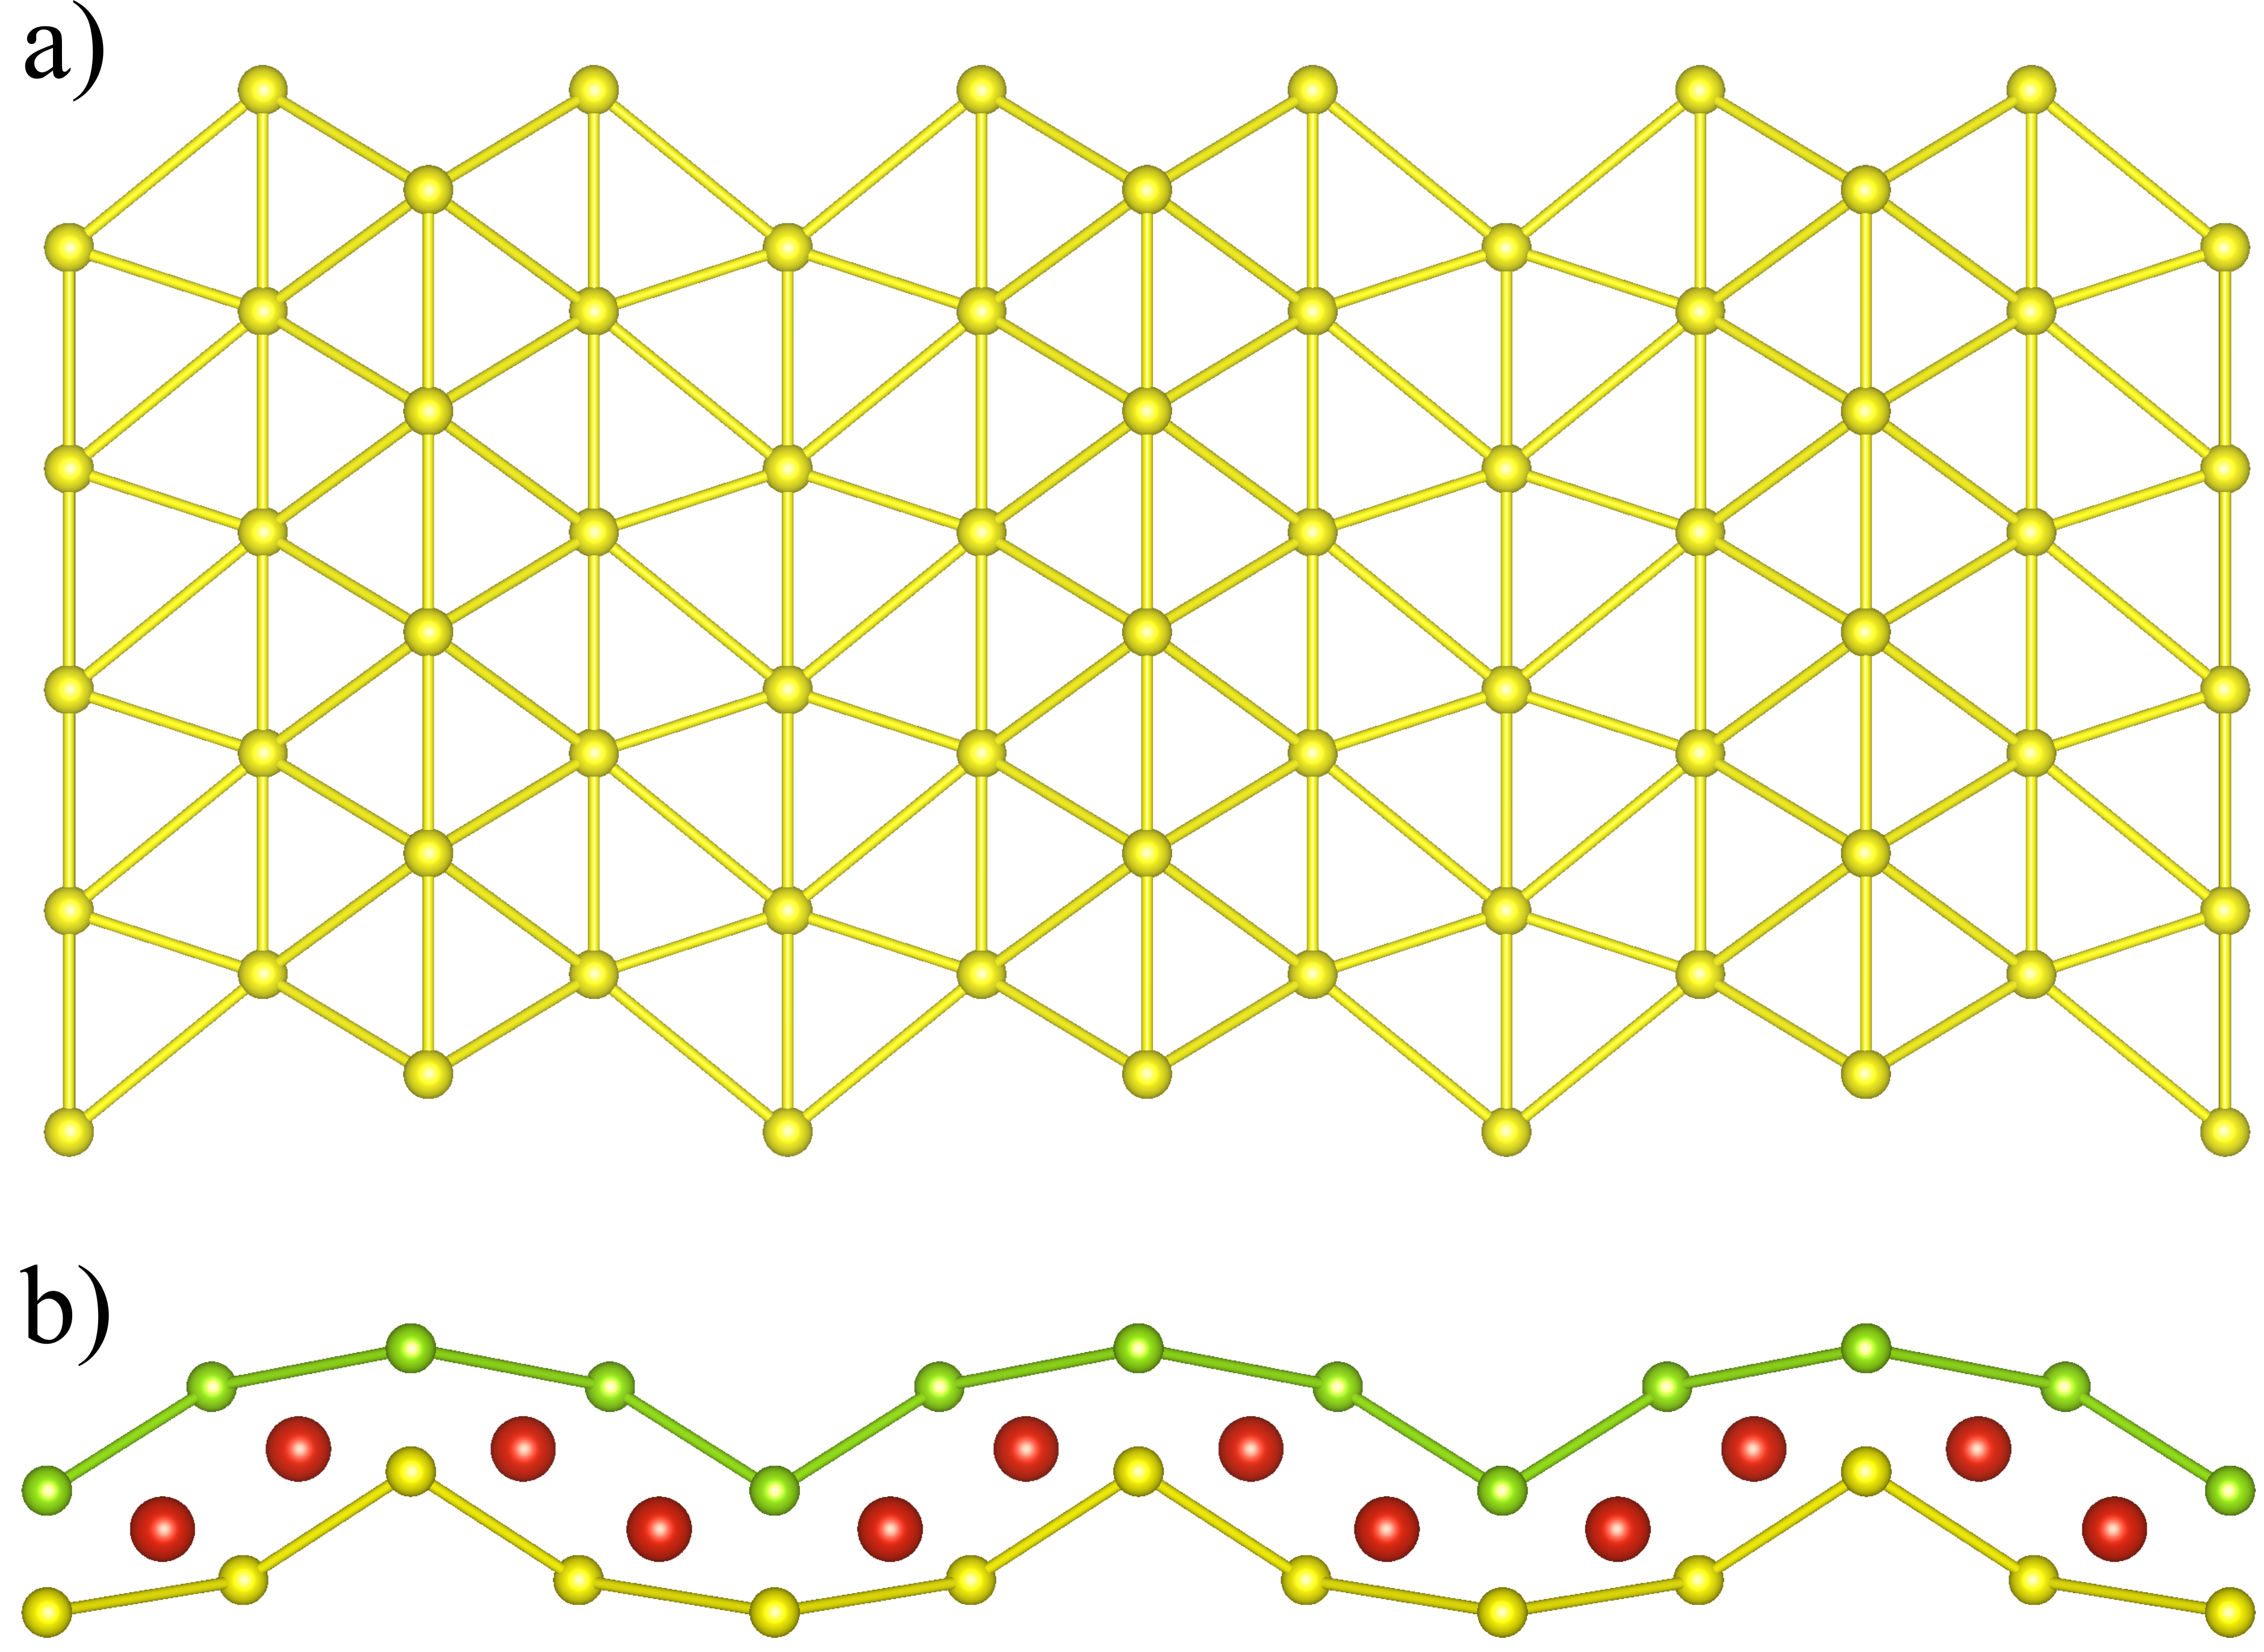
\includegraphics[width=0.5\textwidth]{T_hor_hcb.png} \\
        \caption{The undulated net of chalcogen atom in T-hor structure: top- (a) and side-view (b)}
\label{T_hor_hcb}
\end{figure}


\begin{figure}[H]
	\includegraphics[width=0.8\textwidth]{T_hor_T.png} \\
	\caption{Comparison of T-hor and 1T crystal structures}
	\label{T_hor_T}
\end{figure}

\begin{figure}[H]
	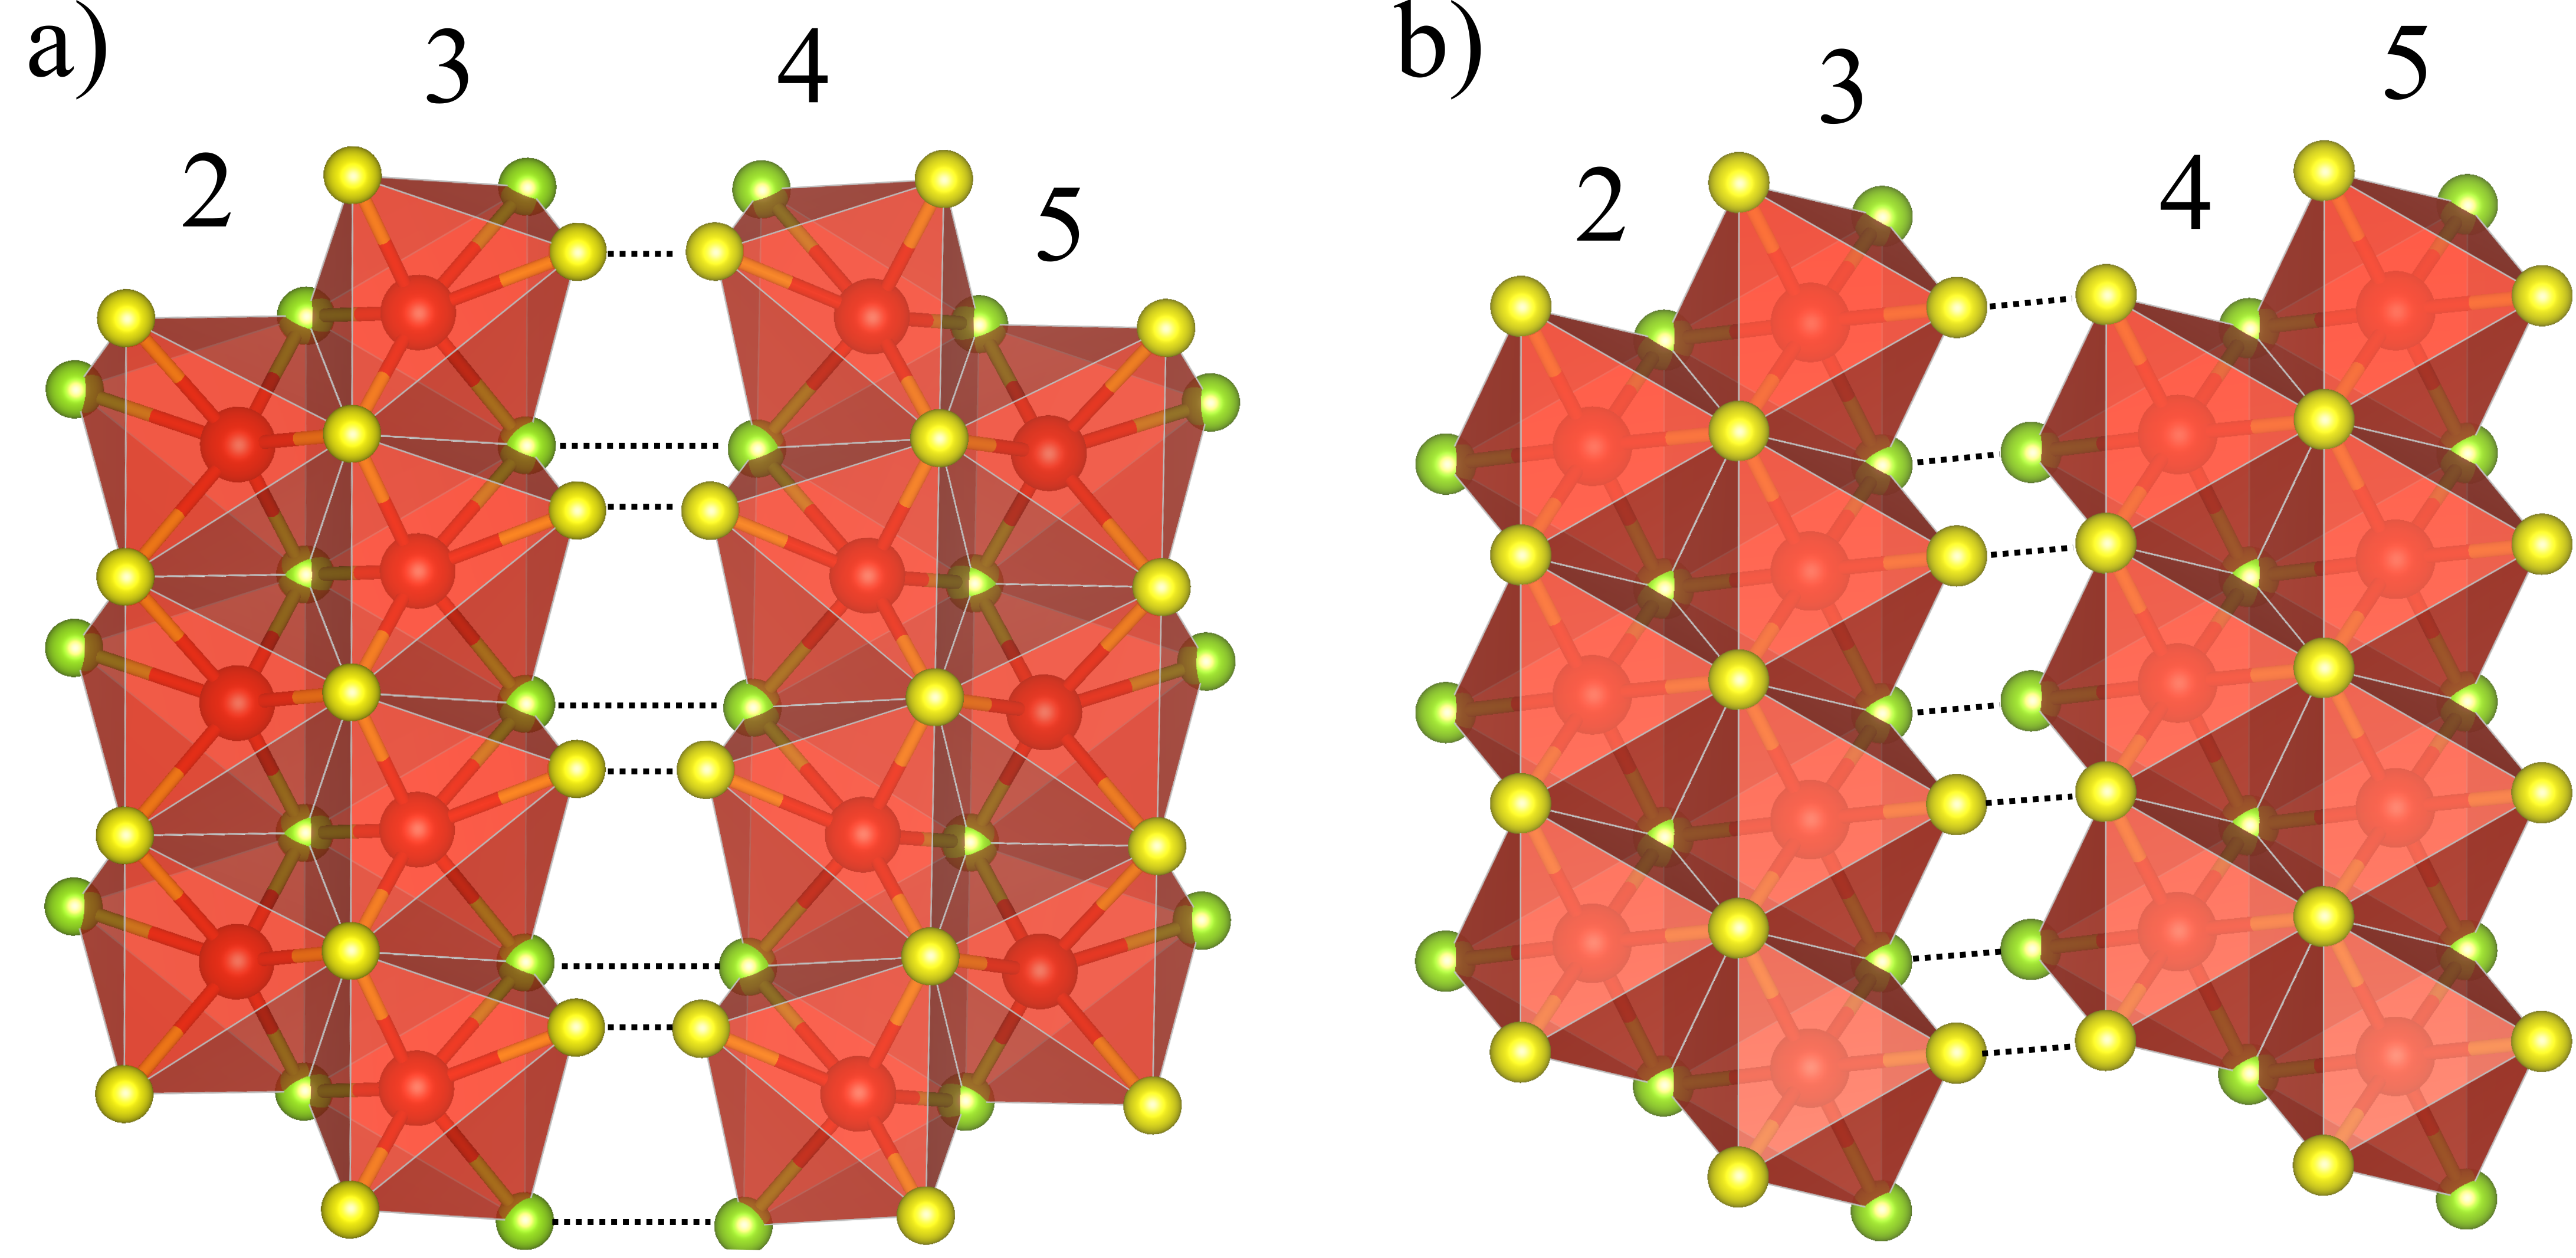
\includegraphics[width=0.7\textwidth]{T_hor_slabs.png} \\
	\caption{Arrangement of double octahedral rows in T-hor (a) and 1T (b) structures; the dashed lines shows the common atoms in the adjacent slabs}
	\label{T_hor_slabs}
\end{figure}

\begin{figure}[H]
	\includegraphics[width=0.5\textwidth]{T_hor_ch.png} \\
	\caption{Comparison of the nets of chalcogen atoms in T-hor (a) and 1T crystal structures }
	\label{T_hor_ch}
\end{figure}

\begin{figure}[H]
	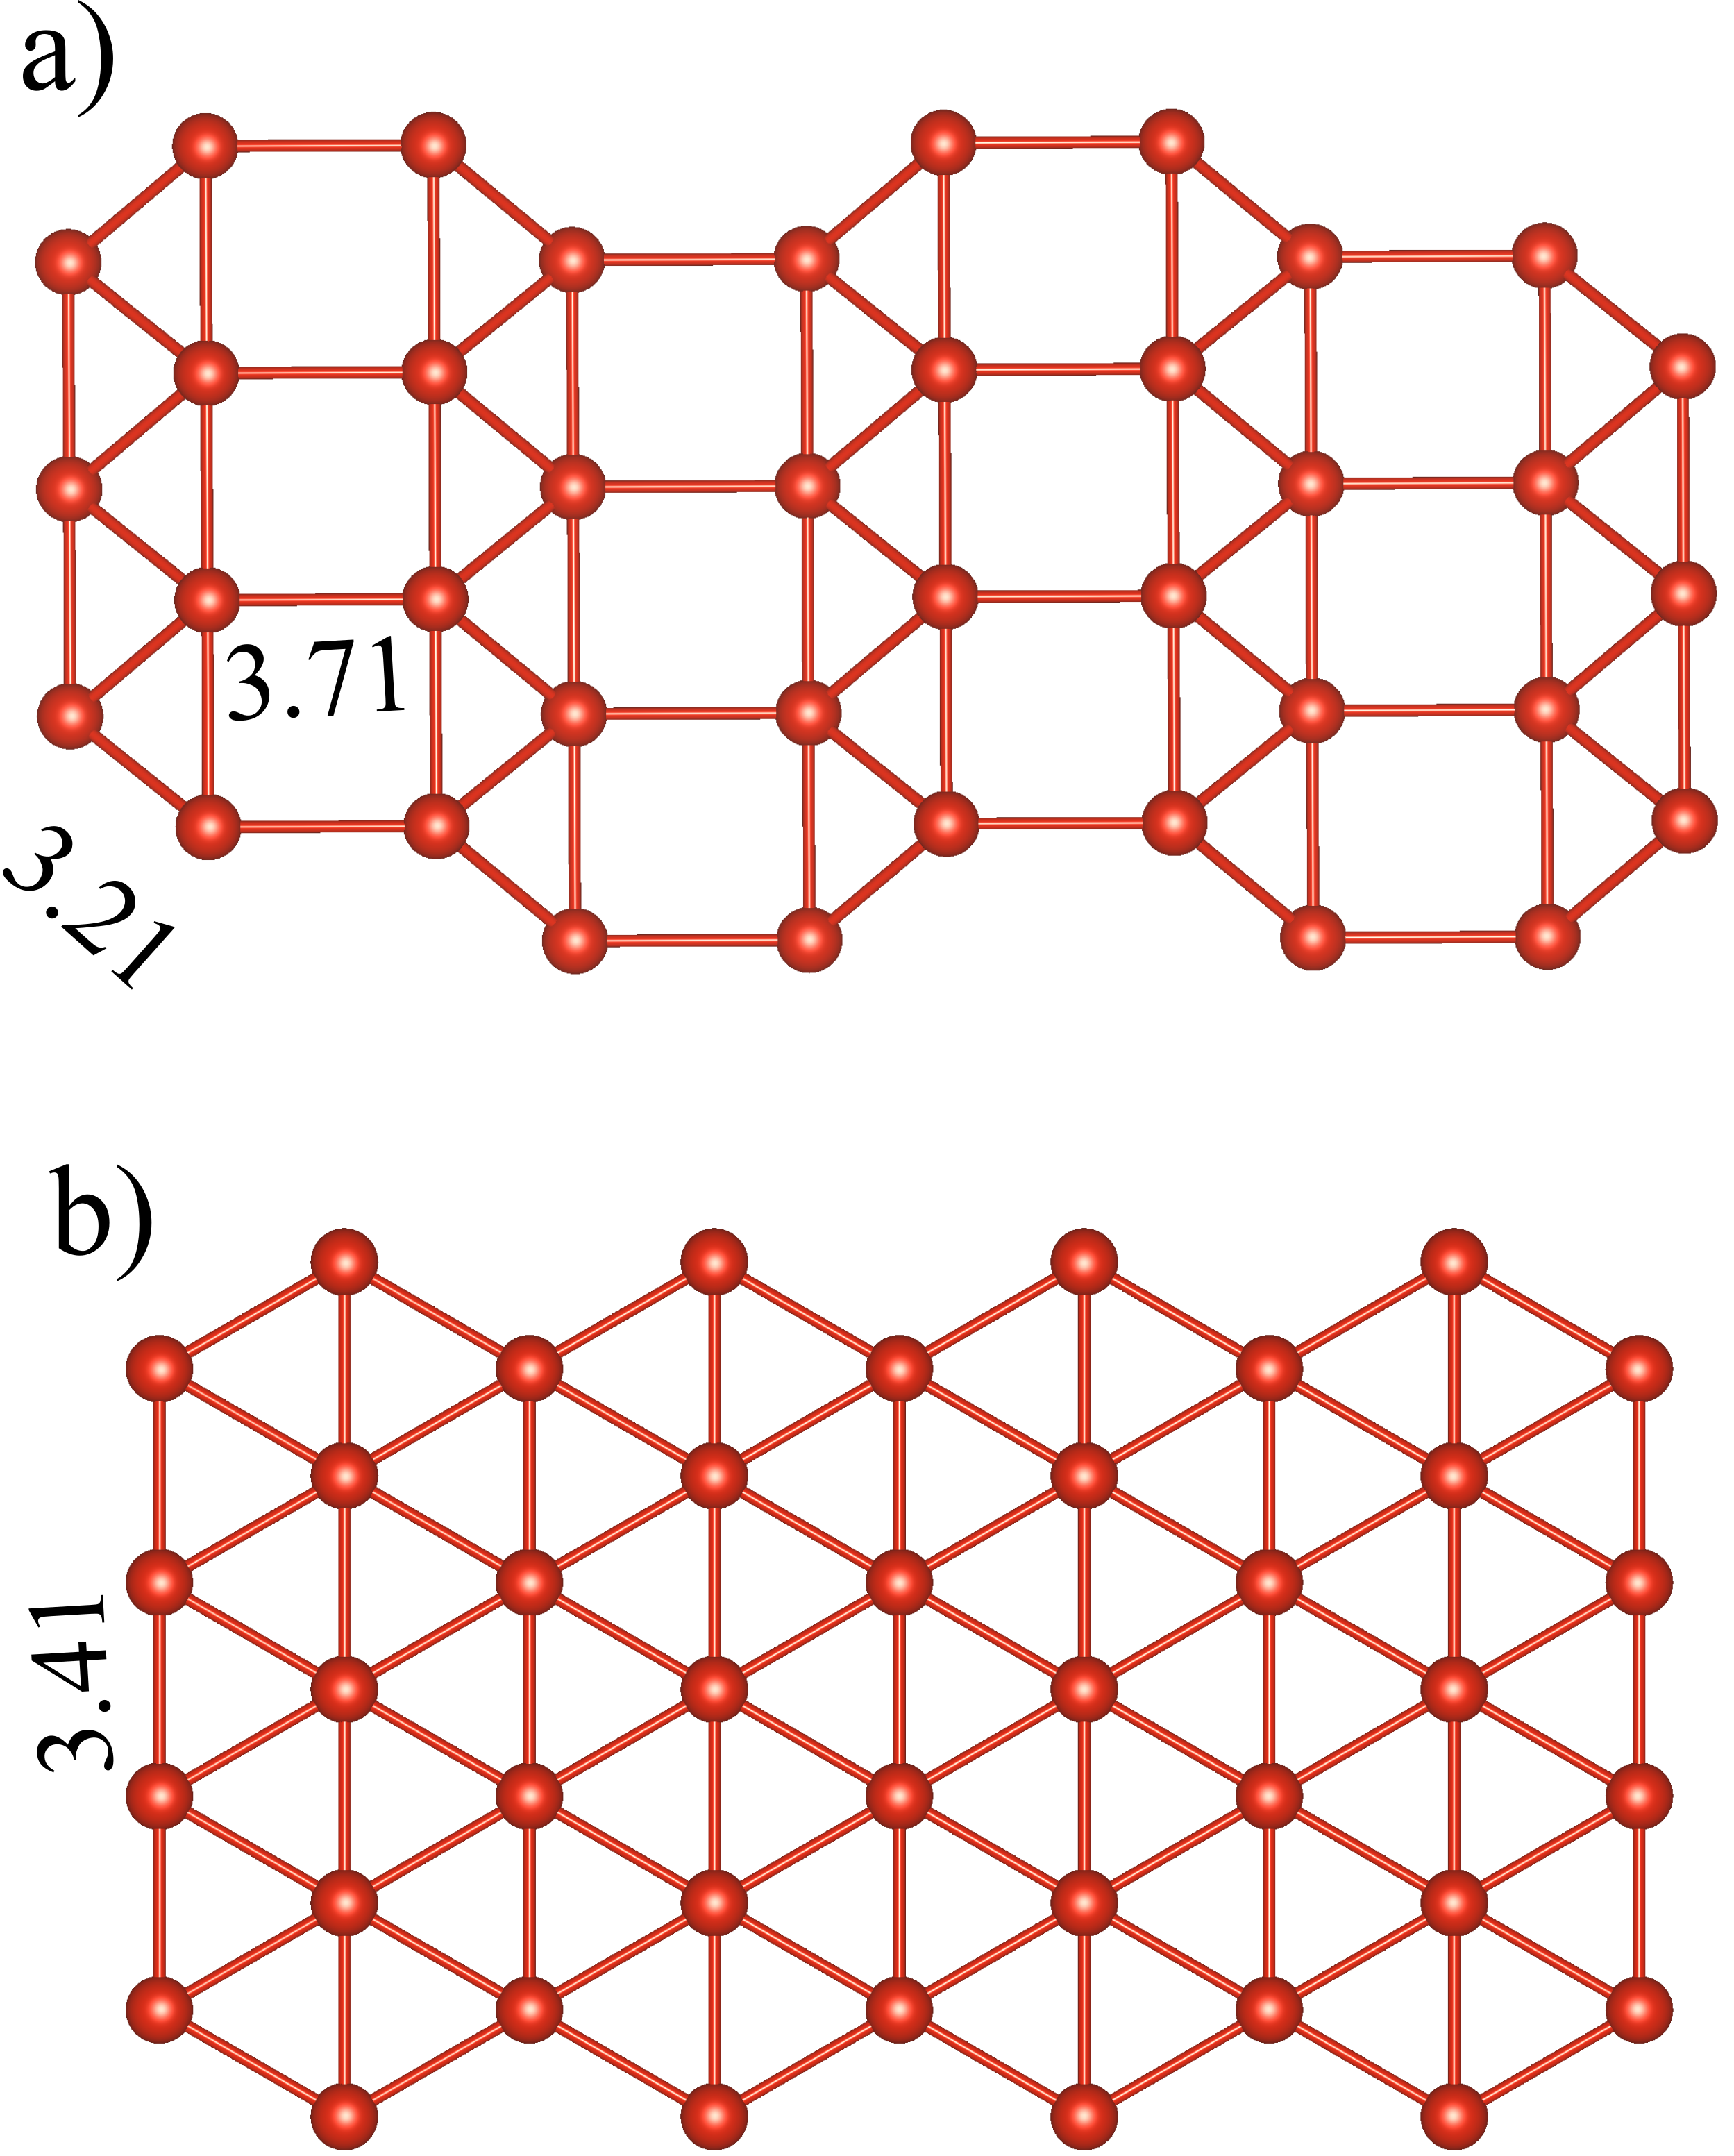
\includegraphics[width=0.4\textwidth]{T_hor_V.png} \\
	\caption{Comparison of the nets of TM atoms in T-hor (a) and 1T crystal structures }
	\label{T_hor_V}
\end{figure}


The structure called AIRSS1 in contrast to T-hor structure is dynamically stable for both VSSe and MoSSe compositions.
For MoSSe composition, the enthlpy ratio is the following: 1T > airrs1 > 1T' > 1H.
The enthalpy of airss1 structure in this case lie inbetween values of enthalpies of 1T and 1T' structures, being more favourable than 1T in nearlu 0.1 eV/f.u.
For VSSe composition -- 1T' < 1T < 1H < airrs1 and airrs1 structure is less favourable than 1H on nearly 0.1 ev/f.u.

The structure airrs-1 can be better described based on the net of transition metall atoms, which forms the well known Kagome lattice\cite{zhang2021_kagome}, observed for transition metals for instance in AV$_3$Sb$_5$ \cite{ortiz2021} and WO3 \cite{gerand1979} compounds.
In both MoSSe and VSSe structures Kagome lattices are not of ideal hexagonal symmetry, there is dispersion in bond lenghts and deviation of bond angles from ideal values of 120\textdegree.
In VSSe  structure, the bond lengths vary in the range 3.07--3.49 \AA\ and bonds between angles – in the rage 115-122.9\textdegree (Figure \ref{airss1_tm}),  in MoSSe bond lengths are in the wide range of 2.78--3.79 \AA, and bond angles are in the range 113.9--125.7 \textdegree.
Airss1 structure of MoSSe is different from VSSe structure in that it is charactersied by the presence of trinagular clusters of transition metall atoms with sufficiently shorter bond lengths.
The bond leghts within clusters vary are equal neraly 2.78--2.81 \AA, while other Mo--Mo bonds are on 0.5--1 \AA longer (Figure \ref{airss1_tm}).
To evaluate the probability for the synhtesis of airss1 structure, using the seed of the some compound with similar kagome lattice of vandium of molybdenum atoms we have performed the automated topological search through the whole ICSD.
As the result 17 structures containing kagome lattice of vanadium atoms have been found.
For comparison we have used Ta2V3Si \cite{Ta2V3Si}, CaV3Sb4 \cite{ CaV3Sb4}, KV3Sb5 \cite{KV3Sb5}, and CoVZr \cite{ZrVCO} crystal structures.
In these crystal structure bond V--V bond length vary in the range 2.43--2.81 \AA.
The pure vanadium and pure molubdenum are characterised by the similar bond length, which are equal to 2.62 \AA\ \cite{vanadium} and 2.72 \AA\ \cite{molybdenum}.
This is close to the lengths of bonds in the mentioned triangular clusters of Mo atoms and sufficiently higher than the lengths of V--V bonds in kagome net of VSSe-airss1 crystal structure.


The net of sulphur atoms in airss1 structure is different from that in 1T and 1H structures (Figure \ref{airss1_s}), but it can be transfromed by the shift shown in the Figure \ref{airss1_s} and subsequent deformations.
Differences of bond angles and bons lengths on airss1 structures of MoSSe and VSSe do not exceed 0.1\AA\ and 1\textdegree.
The deviation of net from the horisontal (001) orientation lies witin $\pm$10\textdegree.

Each transition metall atoms is cooridnated by 5 chalcogen atoms arranged in highly deformed tetragonal pyramid, and this is the only structure amond revealed ones characterising by the coordination number different from 6.
Half pyramids have the composition VS3Se2 and half -- VS2Se3.
The bond distances between transtion metall and chalcogen atom varies in the range 2.26--2.58 \AA\ for VSSe composition and 2.29--2.63 \AA for MoSSe composition.
The pyramids are connected through the common edges in triangular clusters, corresponding to the triangular rings of the mentioned kagome lattice (Figure \ref{airss1_poly}).
Between clusters there are the big holes, corresponds to the centers of hexagonals rings of kagome lattice \ref{airss1_poly}).



\begin{figure}
	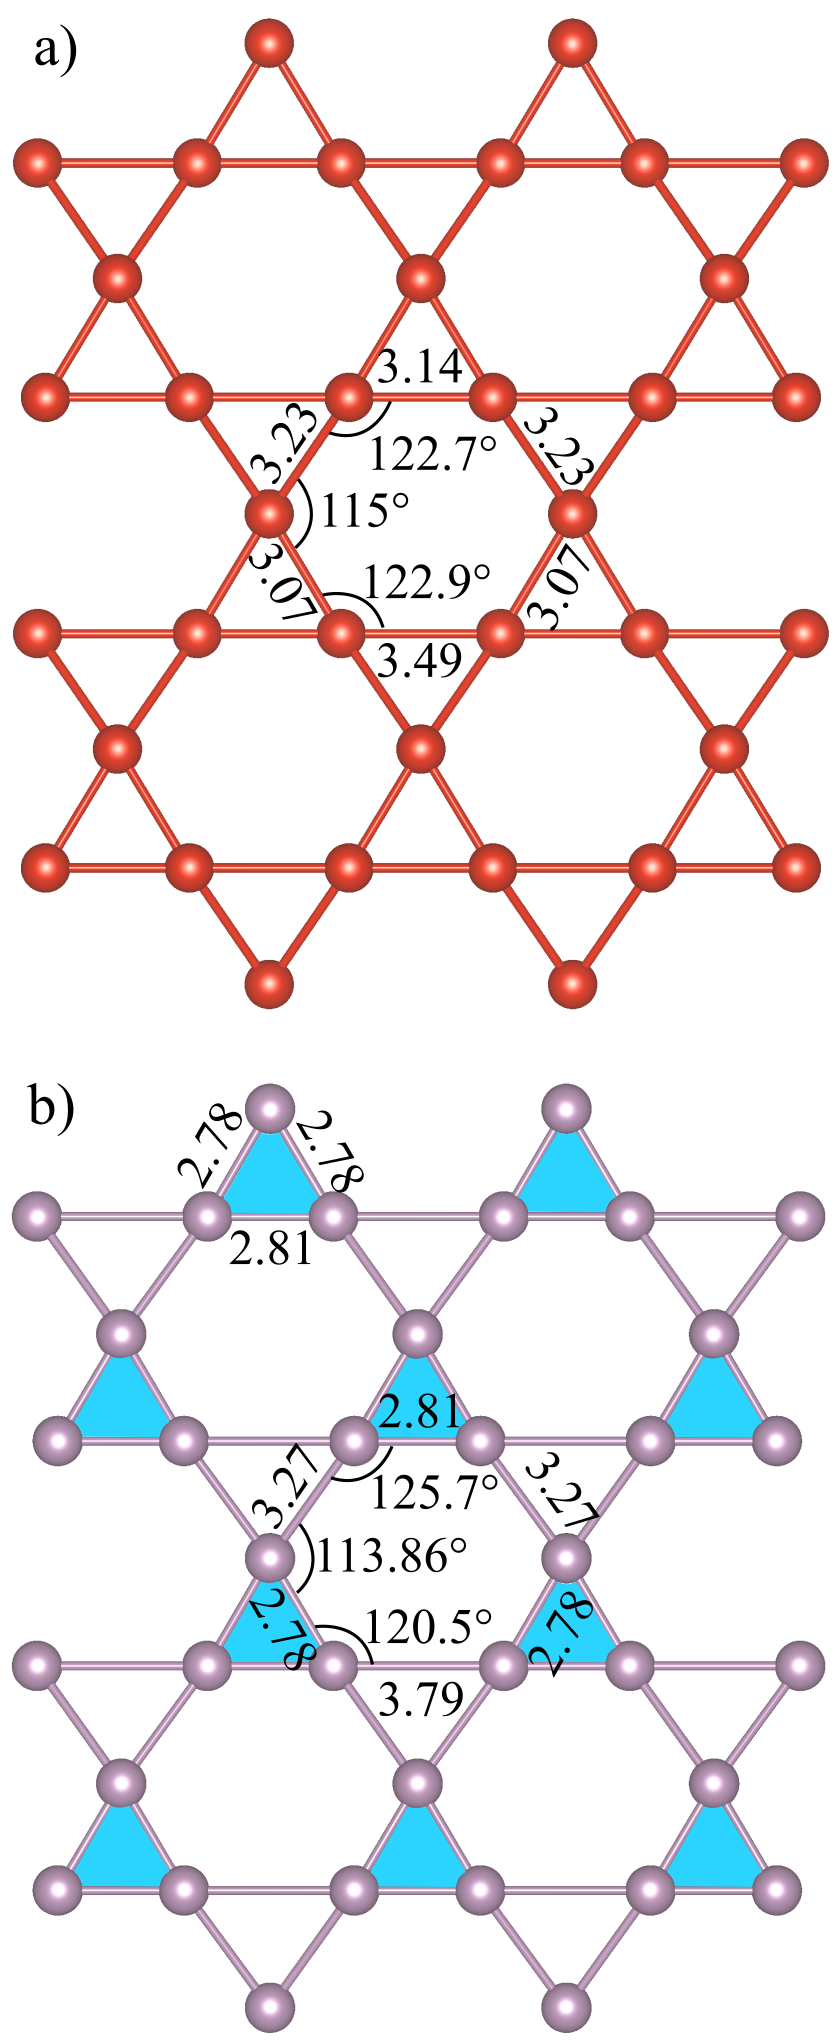
\includegraphics [width=0.5\textwidth]{airss1_tm.png}
	\caption{The Kagome atomic nets of transition metal atoms in VSeSe-airss1 and MoSSe-airss1; tringular clusters of Mo atoms are highlighted in blue} 
\label{airss1_tm}
\end{figure}

\begin{figure}
	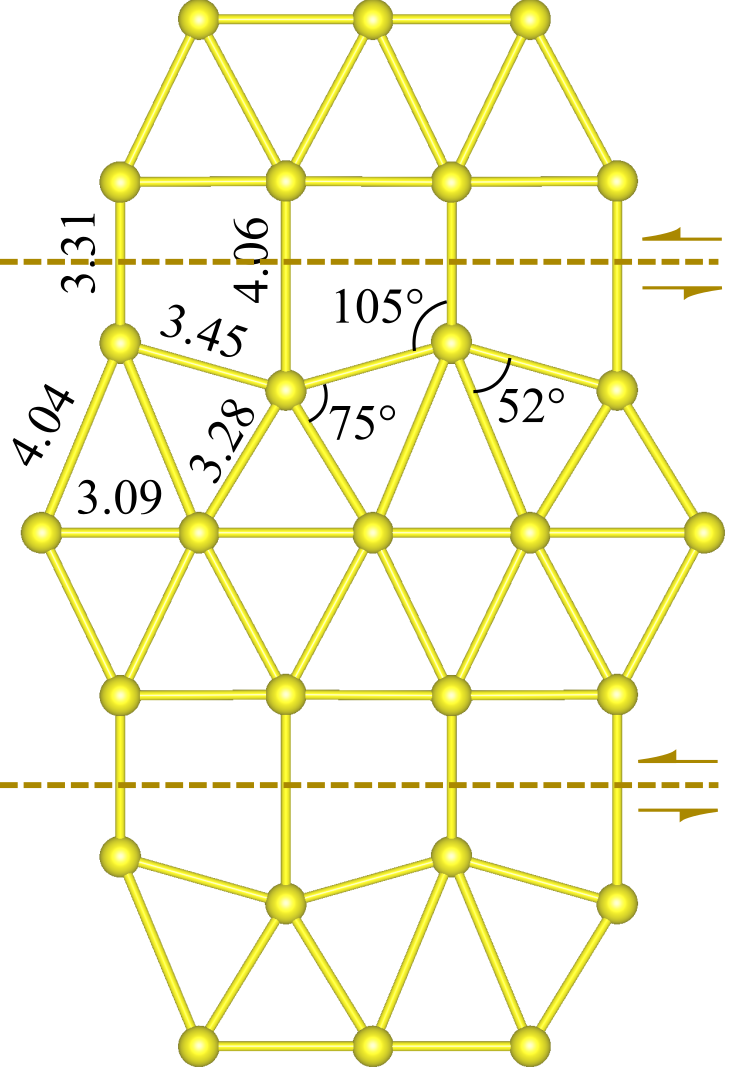
\includegraphics[width=\textwidth]{airss1v_s.png}
	\caption{Net of sulphur atoms in VSSe-airss1 structure; values of interatomic distances are given in \AA; dashed line shows the plane of the shift transforming the net to the hexagonal net of T and H structures}
\label{airss1_s}
\end{figure}

\begin{figure}
	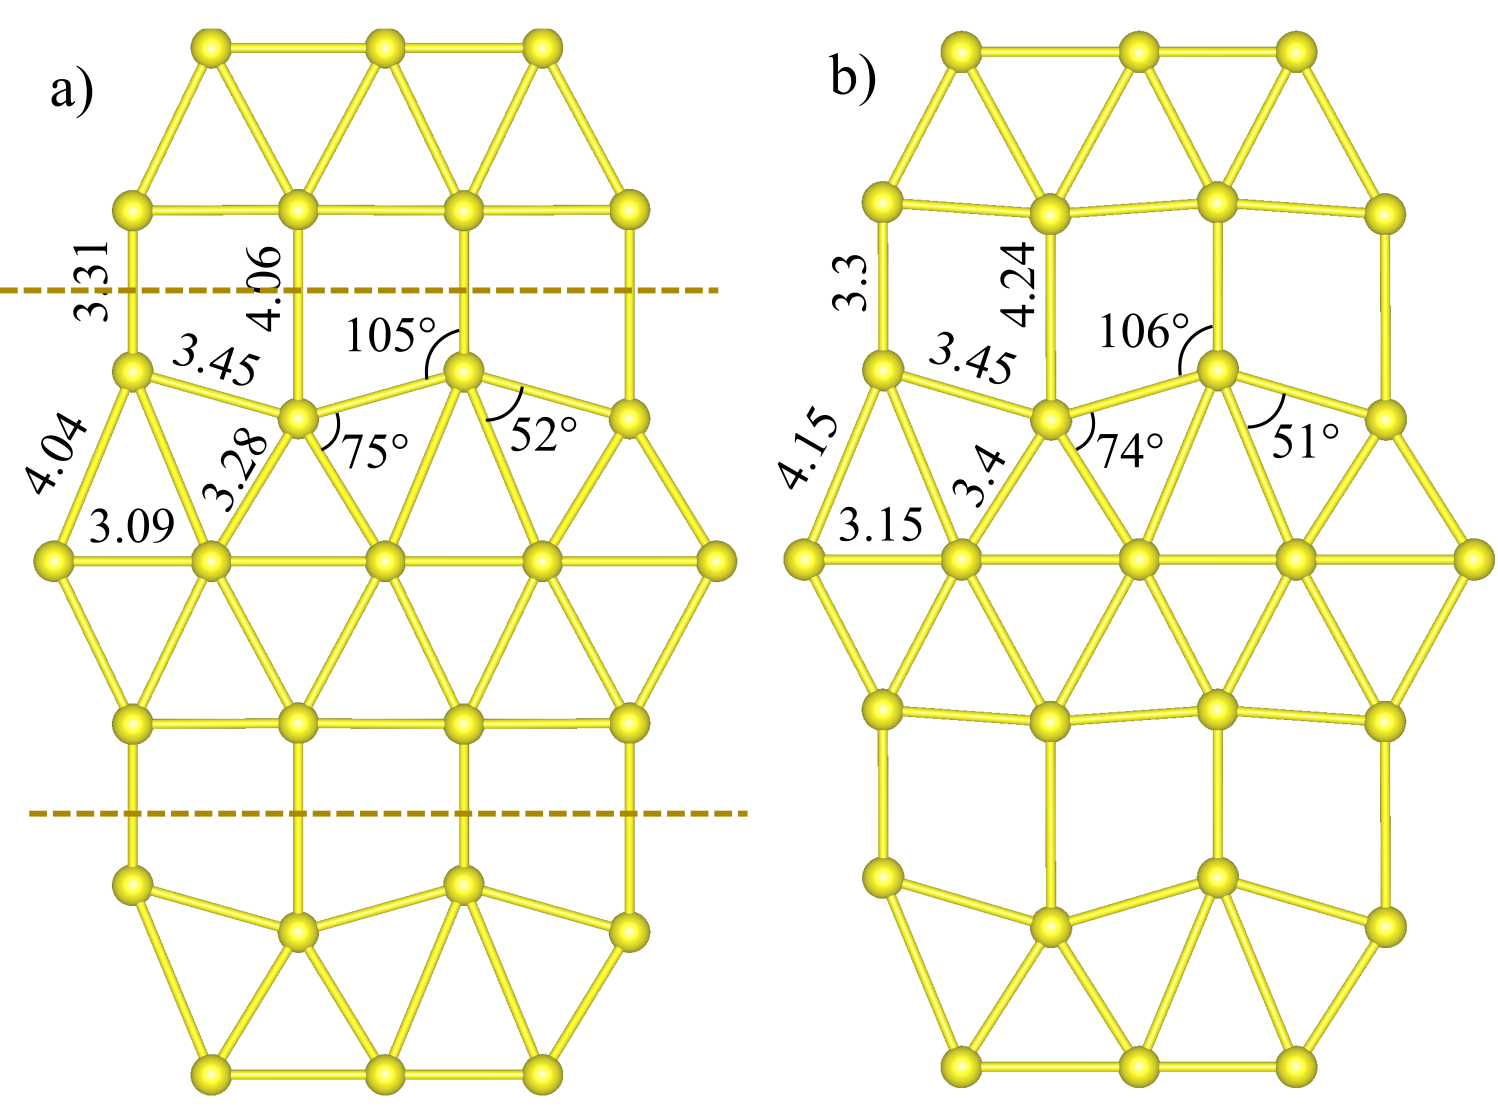
\includegraphics[width=0.5\textwidth]{airss1_s_comp.png}
	\caption{Interatomic distances and bond angles of sulphr nets in VSSe-airss1 (a) and MoSSe-airss1 (b). \bf{Supplementary}}
\label{airss1_s_comp}
\end{figure}

\begin{figure}[H]
        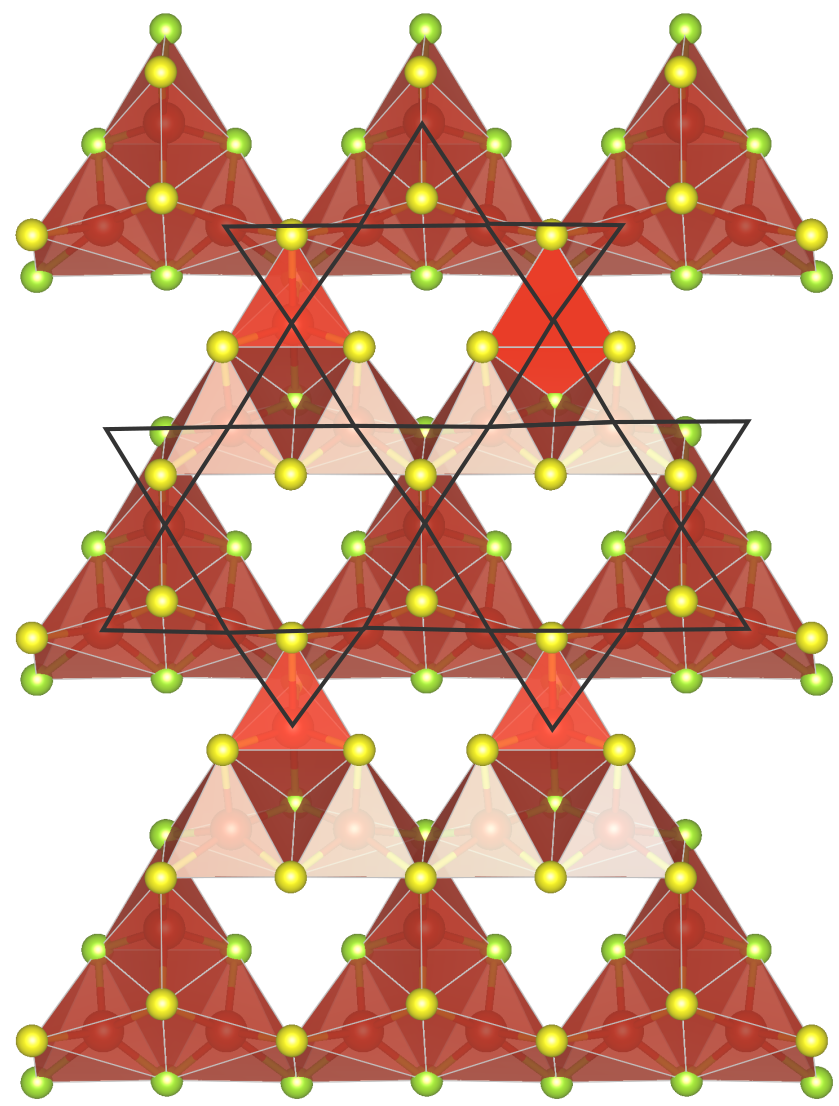
\includegraphics[width=0.5\textwidth]{airss1_v_poly.png}
        \caption{VSSe-airss1 structure with outlined cooridnation polyhedrons around V atoms; kagome lattive of V atoms is highlighted in grey}
\label{airss1_poly}
\end{figure}


%%%%%%%%%%%%%%%%%%%%%%%%%%%
\subsubsection{Test-1, test-2, test-3, and H-hor crystal structures – the derivatives of 1H structure}
%%%%%%%%%%%%%%%%%%%%%%%%%%

To compare topologies of H, fes, and fxt structures and produce similar structures with trigonal prismatic coordination, we present the structures as different fillings of the hexagonal net of sulphur atoms (Figure \ref{H-based}).
H-structure presents the most symmetric chess-board-like filling.
The fes structure can be also considered as the chess-board filling, but with doubled triangular cell, having the form of rhombuses.
After optimisation, these rhombuses trasform in the right squares.
In fxt structure the empty rings (in (001) projection on  (Figure \ref{H-based})) are of two types.
The first have the form of right hexagons and consists of three triangular rings connected through the faces.
The second are primitive triangles.
The optimisation does not sufficiently change the forms of the empty rings, only slightly deforming hexagons.


Three new structures were produced by means of the filling of triangles in the hexagonal net of the sulphur atoms, similarly as it was described for fxt and fes.
We named them abstractly test1, test2, and test3.
We failed to produce new structures obeying the local charge balance, i.e. the structures in which each vertex of the trigonal prism is common for three prisms, as it is in1H, fxt and fes structures.
In the structure test1, each sulphur atom is common for two or four trigonal prisms, in test2 and test3 – for 2, 3, and 4 (Figure \ref{H-based}).
Test3 structure is different from the other structures in that it characterised by the presence of trigonal prisms with two common faces, while in all other structures prisms has no more than one common face.
Optimisation of test3 structure sufficiently affect the arrangement of sulphur atoms.
In the final structure the net of sulphur atoms is not more the hexagonal one.

Presense of common edges and faces of [MoO6] trigonal prisms in fxt, fes, test1, test2, and test3 structure results in shorter Mo--Mo distances in comparison with 1H structure, where prisms have only common edges.
In 1H structure, Mo atoms form regular hexagonal net with all Mo--Mo bonds being equal to 3.25 \AA in 1T' structure -- 2.79 \AA.
In fxt, fes, test1, test2, and test3 structures Mo--Mo distances vary in some range, with formation of Mo--Mo dimer connected by the stronger bonds.
in test1 it equals to 2.9 \AA, in fxt, fes, and test-2 it is in average 2.62 \AA, and test3 is characterised by the shortest Mo--Mo distance of 2.22 \AA\ length with formation of the mentioned dimers.

Phonon dispersion curves show dynamic stability of the test1 and test3 structures (Figure \ref{phon_smose}).
Enthaliies of these structures are nearly 0.2--0.4 eV/f.u. higher then the enthlpy of 1T structure for SMoSe composition and .
Test-1 structure can be considered as polysynthetically twinned 1H structure through the plane \{110\}, which is horisontal in Figure \ref{H-based}.
This structure can be produced on the boundary of \{110\} between two grains.
Similarly fxt structure was suggested as the grin boundary structure \cite{}.

\begin{figure}[H] \centering
        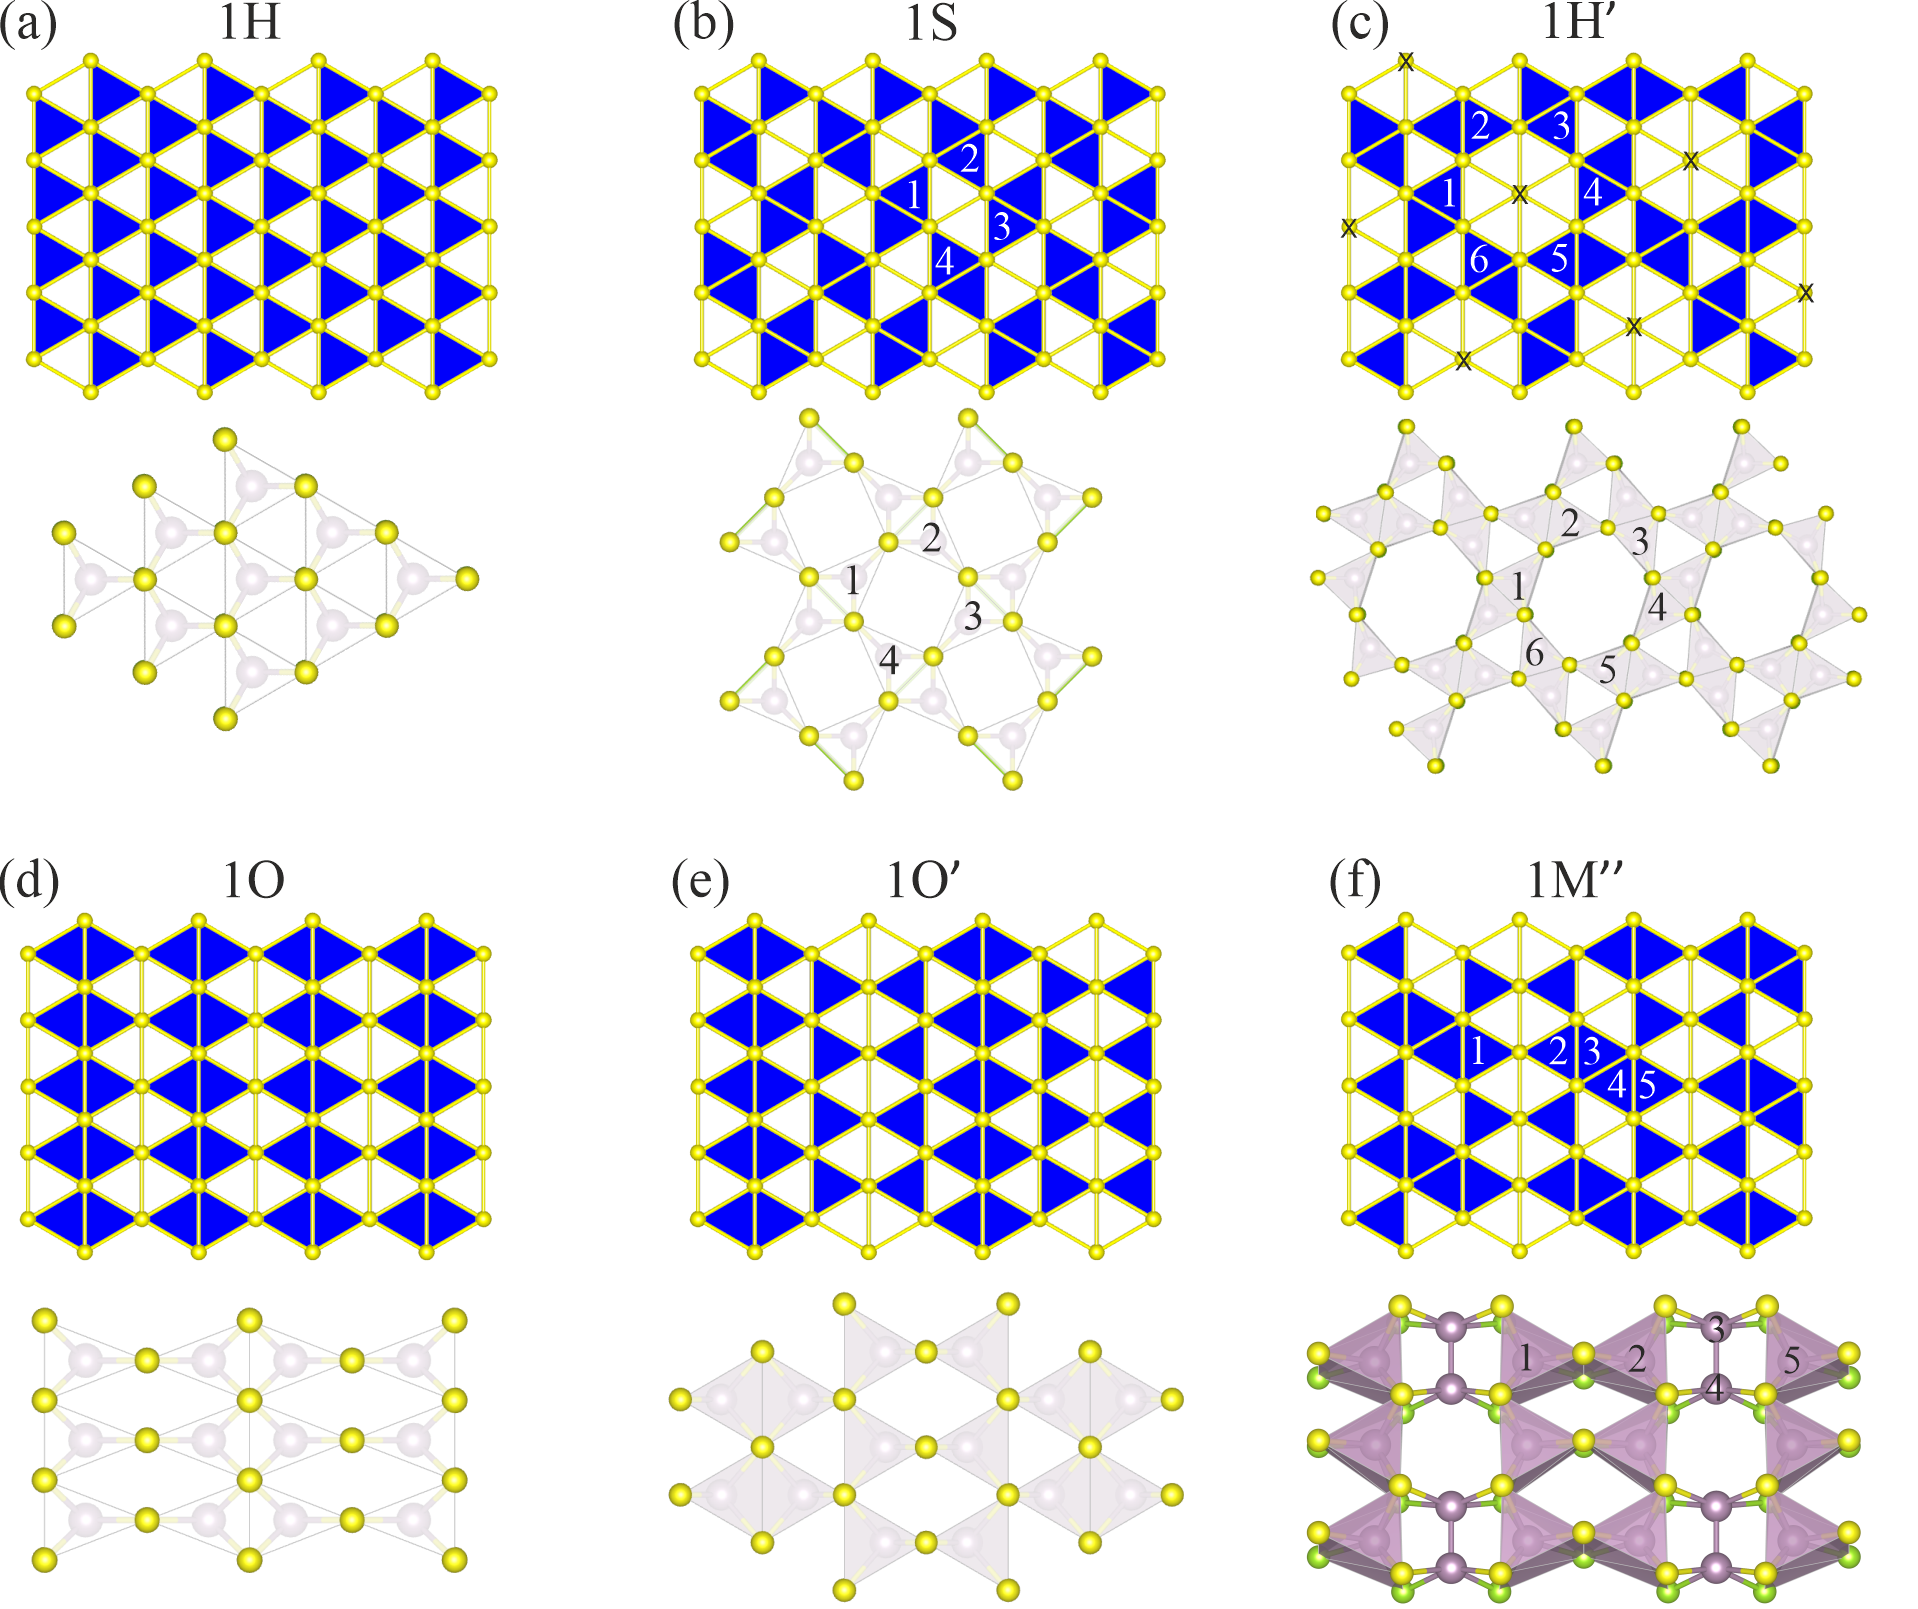
\includegraphics[width=\textwidth]{H-based.png}
        \caption{The initial and optimised structures of SMoSe. Numbers on polyhedra are given to show the same fragment before and after the optimisation.}
 %! Для test-3 нужно нарисовать пунктирную связь Mo--Mo.
\label{H-based}
\end{figure}


Another structure characterising by the trigonal prismatic coordination was found by means of the USPEX package.
It is sufficiently different from 1T structure and its derivatives in that the three-fold axes of trigonal prisms are parallel to the plane of monolayer.
As the result the rings of the net of chalcogen atoms became the square ones (Figure \ref{H_hor}.
This structure was called 1H-hor (abbreviation from the analogue of 1H with horisontal trigonal prisms).
Crystal structure of 1H-hor phase is characterised by monoclinic symmetry $Pm$ (\#6), with $\beta$ angle equals to 98.67\textdegree.
The $a$ and $b$ axes parallel to the plane of the layer are orthogonal and $a$ is almost to times greater than $b$ (Table \ref{t:str})

\begin{figure}[H]
	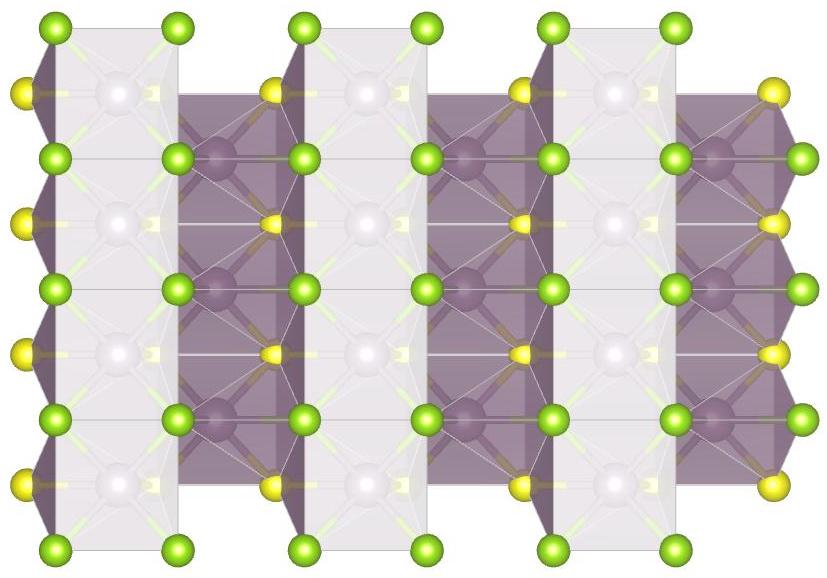
\includegraphics[width=0.5\textwidth]{H_hor_1.jpg} \\
	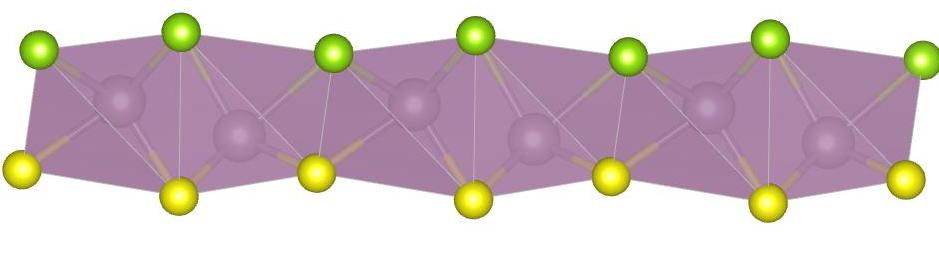
\includegraphics[width=0.45\textwidth]{H_hor_2.jpg}
	\caption{H-hor crystal structure perpendicular and along the layer.}
\label{H_hor}
\end{figure} 





%%%%%%%%%%%%%%%%%%%%%%%%
\subsubsection{ Airss-3 – the mixed layers of TM and chalcogene}
%%%%%%%%%%%%%%%%%%%%%%%

The structure in which TM are sufficiently shifted from the center towards upper and bottom layer was revealed for SVSe composition with AIRSS code and have been called airss-3 (Figure \ref{airss-3}).
V atoms in this structure are characterised by the coordination numbers of five and six, and coordination polyhedron have the forms of tetragonal pyramid and trigonal prism respectively.
Structure can be presented as the combination of double chains, one is with the subhorisontal faces of [SV4] composition in the upper layer and another is with subhorisontal faces of [SeV4] composition in the bottom layer.
Polyhedrons are connected through the common edges.
Each tetragonal pyramid share six out of eight common faces and trigonal pyramid – three out of nein.

\begin{figure}[H]
        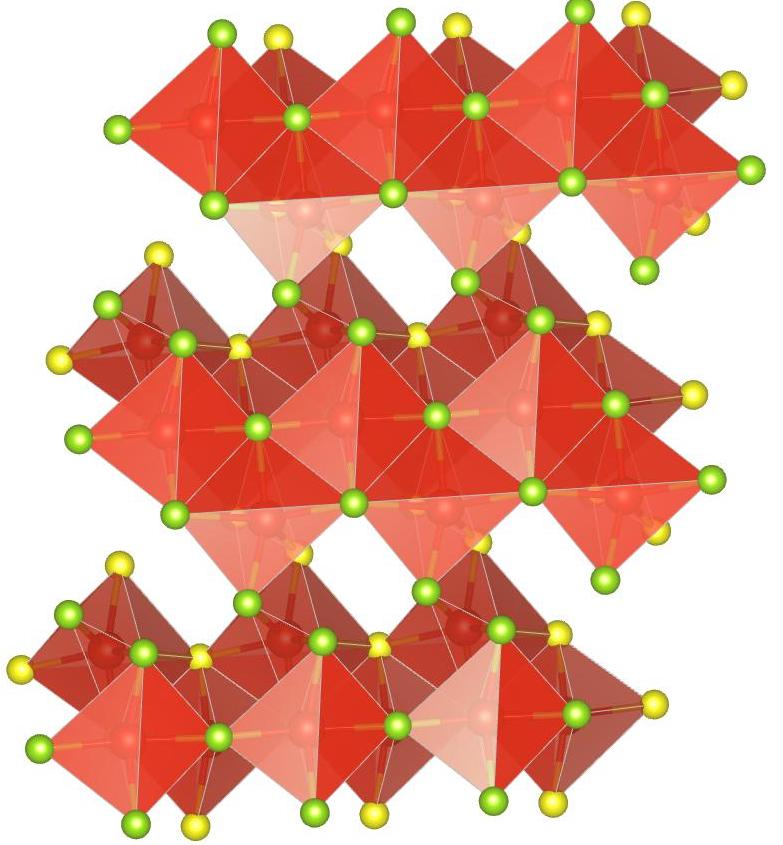
\includegraphics[width=0.5\textwidth]{airss-3-1.jpg} \\ \vspace{3mm}
        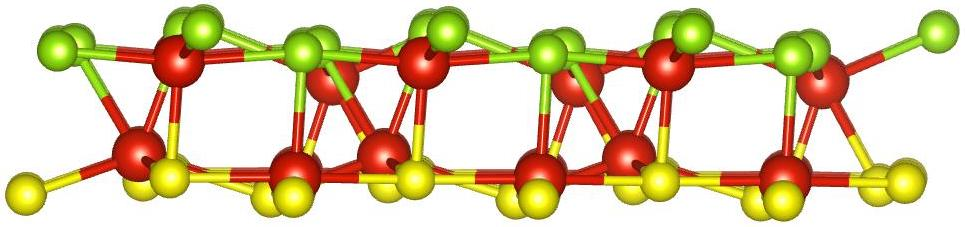
\includegraphics[width=0.5\textwidth]{airss-3-2.jpg}
        \caption{AIRSS-3 structure with V atoms shifted towards the planes of chalcogenes.}
\label{airss-3}
\end{figure}


%%%%%%%%%%%%%%%%%%%%%%%%
\subsection{The uniquenes of the new structures}
%%%%%%%%%%%%%%%%%%%%%%%

To answer the question, whether the found structures are unique or there are similar representatives in ICSD we have performed topological search.
The obtained results have shown that all the found structures, except of H-hor, are unique and similar structures are not found in ICSD.
The same is true about the earlier known fxt and fes structures, similar structures of which have not also been found. 
The H-hor structure belong to the same kgd topological type as the T structure.
This means that one structure can be transformed into another without breaking the bonds.
However the geometrical difference of H-hor and T structures is sufficient and transformation of one structure into the other requires changing of the coordination polyhedron from trigonal prism to octahedron.

Comment:
Although TOPOS have not found such a structures, some analogues exist.
Interestingly, we note that this structure resembles the structure of the recent experimentally identified monolayer C2N-h2D[J. Mahmood, E. K. Lee, M. Jung, D. Shin, I. Jeon, S. Jung, H. Choi, J. Seo, S. Bae, S. Sohn, N. Park, J. H. Oh, H. Shin, and J.
Baek, Nat. Commun. 6, 6486 (2015)]





\subsection{Crystal field splitting}

The crystal field theory proceeds from the fact that the nature of ligands and their location around the central ion (symmetry of the complex) reduce the degeneracy of d-orbitals and change their energy. As all investigated structures consist of transition metal atoms surrounded by ligands (chalcogen atoms), the presence of the ligands splits the d-electrons levels depending on local symmetry. Thereby the correlation between structure and electronic properties can be interpreted in terms of crystal field theory. According to crystal field theory, in an octahedral environment (1T polymorph), the d-shell splits into a low-energy triplet (t2g) and a high-energy doublet (eg). In a trigonal prismatic geometry (1H), the low-energy triplet further splits into a doublet and a singlet [https://doi.org/10.1088/2053-1583/ab0188]. The two polymorphs of MoS2 have distinct electronic properties, the 1H-MoS2 is a semiconductor and the 1T-MoS2 is metallic. The fes-MoSSe despite the prismatic environment of TM atom becomes a semi-metal [10.1016/j.physe.2020.114485 , 10.1039/D1NA00112D] and fxt Mo and W based TMDs are gapless semiconductors or, alternatively, semimetals [10.1103/PhysRevB.93.035442]. The proposed structure airss-1 is characterized by a distorted trigonal bipyramidal local environment of the TM atom, which should make these structures more metallic due to degenerate d-orbitals. The squire pyramidal environment in airss-3 with the bare square facet of the pyramid can apply this structure for molecular sorption which makes materials in such structure perspective for sensoric and catalytic applications. In addition, despite the fact that the surroundings of metal atoms have a prismatic environment in the geometries fxt and fes make metal atoms available for use in chemical applications due to the steric factor.

The variation of structures dictates variation electronic properties based on different d-splitting and electron filling of d-orbitals which makes it possible to manipulate electronic properties through phase transformation.


\bibliography{2d}
\bibliographystyle{CGD}


\end{document}


Comment. 
fes structure denoted as S-MS2 in \cite{tang2021_smose}.
fxt structure denoted as H' in \cite{ma2016_h'}.
Similarly there is T' – deformed T-phase.
We can follow this notation, designating our phases by symmetry with addition of '.


2.43--2.56 -- Ta2V3Si
2.81475		-- CaV3Sb4
2.74090		--KV3Sb5
2.53143		--CoVZr
2.61895		-- Vanadium \cite{vanadium}
2.72019		-- molybdenum \cite{molybdenum}